\documentclass[11pt]{report}
\usepackage{standalone}
\usepackage{tikz}
\usetikzlibrary{positioning,arrows,decorations.pathreplacing,calc,fit}

\usepackage{fouriernc}

\usepackage[T1]{fontenc}
\usepackage[utf8]{inputenc}
\usepackage{graphicx}
\usepackage[a4paper]{geometry}
\geometry{verbose,tmargin=2cm,bmargin=2cm,lmargin=3cm,rmargin=3cm,columnsep=0.8cm}
\usepackage{multicol}
\usepackage{float}
\usepackage[portuguese]{babel}
\usepackage{amsmath}
\usepackage{bytefield}

\usepackage{multirow}
\usepackage{listings}
\usepackage{minted}

%translation hacks
% po4a: environment tikzpicture
% po4a: environment minted []{}
% po4a: verbatim environment minted
% po4a: environment bytefield

%trick po4a into not including standalone files as translatable part
\newcommand{\dtinput}[1]{\input{#1}}

\begin{document}

\newcommand{\hbus}[1]{\includegraphics[scale=#1]{../media/hbus}}
\newcommand{\hbuscommand}[1]{\textbf{#1}}
\definecolor{bg}{rgb}{0.95,0.95,0.95}

%define a dummy command so included files can know that they are being included by master document
\newcommand{\HBUSDOCMASTER}{YES}

\begin{center}
\topskip0pt
\vspace*{\fill}
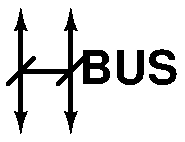
\includegraphics[scale=3]{../media/hbuslogo.pdf}

\huge \textbf{Especificação e exemplos de uso}\\
Versão preliminar 1.1.1
\vspace*{\fill}

Bruno Morais

brunosmmm@gmail.com

\end{center}

\pagebreak

\tableofcontents

\section{Log de mudanças}

\subsubsection{Versão 1.2.1}

\begin{itemize}

\item Definição do objeto de broadcast de informações

\end{itemize}

\subsubsection{Versão 1.2}

\begin{itemize}

\item Introdução do conceito de objetos especiais do mestre

\end{itemize}

\subsubsection{Versão 1.1.1}

\begin{itemize}

\item Modificações para guiar mestre na interpretação dos dados de objetos
\item Novas flags para os objetos de escravo, incluindo a introdução de objetos escondidos (invisíveis) e declaração do tipo de dados contido no objeto
\item Implementação inicial do sistema de eventos internos HBUS para o escravo
\item Re-estruturação das pastas e arquivos padrão

\end{itemize}

\subsubsection{Versão 1.1}

\begin{itemize}
\item Introduzidas medidas para garantir autenticidade do mestre
\item Introduzido o conceito de privacidade do objeto
\item Adicionadas novas instruções para o ANEM-HBUS
\end{itemize}

\subsubsection{Versão 1.0}
\begin{itemize}

\item Versão inicial

\end{itemize}

\part{Concepção e hardware}

\chapter{O barramento HBUS}


Detalhes do barramento e processo de concepção.

\section{O que é HBUS e o seu objetivo}

O barramento HBUS é uma especificação desenvolvida para explorar possibilidades de automação doméstica, daí seu nome, derivado de \textit{Home Bus}.

A especificação contém definições tanto de hardware e software para acomodar a troca de informações entre os dispositivos que participam de uma rede de automação doméstica.

Além de ser uma ferramenta desenvolvida para a exploração e aquisição de conhecimento na área de automação, o conjunto de soluções aplicadas mostrou-se muito capaz de funcionar de forma coerente.

\section{O processo de concepção inicial}

Antes de mais nada, é necessário pensar um pouco para que o projeto tenha sentido e seja realizável.

\subsection{A filosofia de alocação de recursos}

Todo o projeto foi pensado de forma a ser flexível e as especificações podem ser atendidas por uma gama enorme de plataformas e meios físicos de transporte de dados.

No entanto, as definições de operação, tanto em termos de software quanto em escolha de hardware voltaram-se sempre para a economia de recursos. Isto reflete em pouco uso do canal de comunicação, pouco uso de memória nos dispositivos hóspedes do software e etc.

\subsection{Análise de requisitos}

O projeto é voltado para uso em ambiente residencial. A automação residencial pode englobar muitos dispositivos, mas  consiste principalmente em controlar aplicações utilizadas no dia-a-dia, como iluminação ambiente outros.

Além do controle, muitas vezes também é desejável a obtenção de informações sobre o estado físico do ambiente, como temperatura, nível de luminosidade, umidade relativa e etc.

Muitas vezes deseja-se controlar e/ou obter informações em pontos bastante distantes entre si. Por isso é necessário selecionar um canal de comunicação que seja capaz de enviar e receber dados de forma robusta considerando essa possível distância entre os dispositivos de controle.

Um outro ponto a se considerar é que muitas vezes esses dispositivos realizam tarefas que apresentam baixo consumo de potência. O barramento então deve ser capaz de fornecer essa potência remotamente, eliminando a necessidade de alimentação do dispositivo de controle no local. Isto elimina uma série de problemas e simplifica o processo.

No entanto, não é eliminada a possibilidade de necessidade de uma potência que o barramento não pode suportar e o desenvolvedor do dispositivo é livre para realizar a alimentação local, mas devem ser tomados cuidados para garantir o isolamento e segurança.

Também é necessário levar em consideração o dimensionamento do sistema. Uma residência pode conter um número alto de dispositivos para a sua automação, porém esse número muito dificilmente chega à casa das centenas, visto que diferentemente de um ambiente industrial, uma residência tem um tamanho apenas suficiente às necessidades de conforto dos habitantes.

\section{Adequação à realidade e tecnologias disponíveis}

Levando em consideração os requisitos apontados anteriormente, realizou-se uma pesquisa para selecionar as tecnologias a serem utilizadas nesta aplicação. 

Este documento tornaria-se extenso e cansativo caso apresentasse todas as alternativas que foram pesadas e numa sincera tentativa de fazer com que o leitor não abandone-o nem salte aleatoriamente pelo texto para chegar ao fim mais rapidamente, essas informações redundantes foram suprimidas.

\subsection{O canal de comunicação}

A importância da seleção de um canal de comunicação adequado já foi mencionada.

O barramento HBUS trafega todos os seus dados sobre um par trançado de fios de cobre, seguindo o padrão \textbf{TIA-485}, mais conhecido como \textbf{RS-485}.

Este é um padrão que especifica as características elétricas dos dispositivos de transmissão e recepção, em uma rede multiponto com até 32 dispositivos conectados. É possível alcançar distâncias de até 1,2km com uma velocidade de transmissão de 100 kbits/s.

\subsubsection{HBUS e RS-485}

O padrão HBUS utiliza um canal \textit{half-duplex} com velocidade de 100 kbits/s. A velocidade é mantida baixa por questão de maior resistência a ruído e interferências externas, além de facilitar o uso de dispositivos com baixa performance.

A escolha do padrão define o comportamento da comunicação entre os dispositivos. Este é um sistema multi-ponto, ou seja, todos os dispositivos estarão conectados em paralelo escutando e transmitindo no mesmo canal. 

A arquitetura mais óbvia é a adotada pelo padrão HBUS: há um mestre de barramento e todos os dispositivos remotos são escravos.

Procurando fazer com que o canal de comunicação esteja livre o maior período de tempo possível, uma vez que o sistema é \textit{half-duplex}, por definição os escravos não podem iniciar comunicação no barramento, embora isto seja possível e previsto pelo protocolo de comunicação, como será visto mais adiante. Apenas o mestre deve inciar as comunicações e a única exceção para este comportamento é a ocorrência de interrupção por parte do escravo.

\subsection{Sinais no barramento físico}

O barramento HBUS contém os sinais para a comunicação e também alimentação remota dos dispositivos como já discutido. Além disso, o barramento contém mais um sinal, que é o sinal de interrupção.

Este sinal dá aos dispositivos remotos a capacidade de chamar o mestre à atenção devido à algum tipo de evento especial. O procedimento é discutido em detalhes mais adiante.

\section{Exemplo de uso em ambiente residencial}

\begin{figure}[H]
\centering
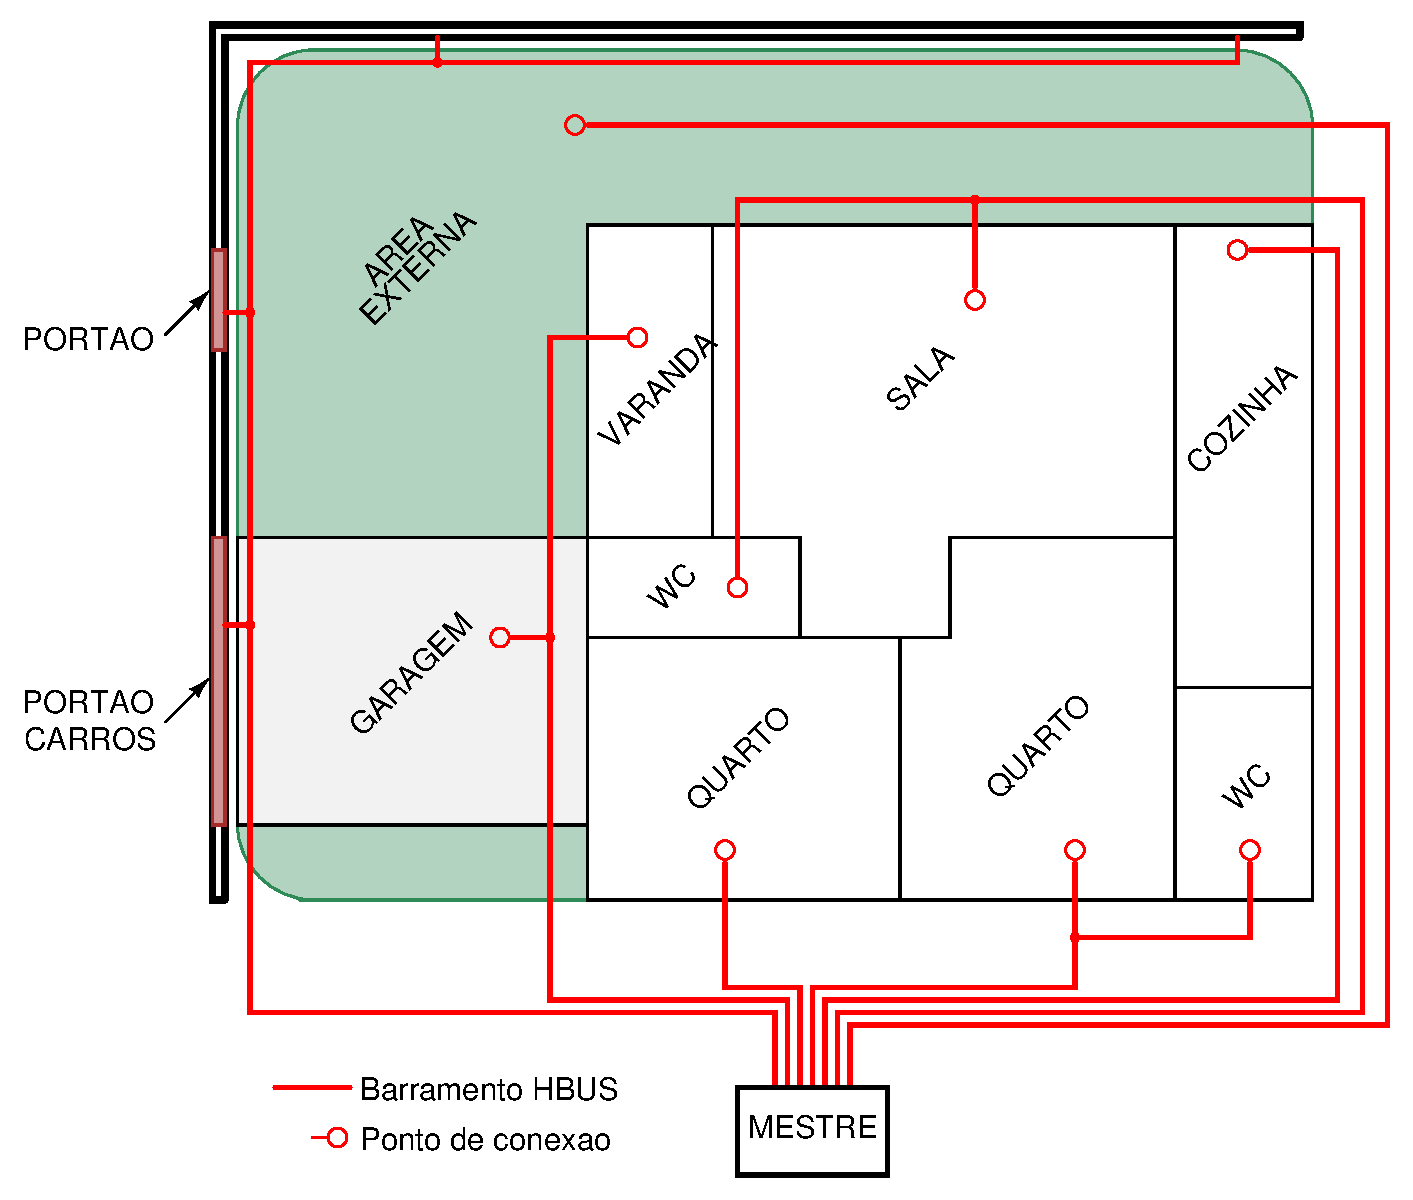
\includegraphics[scale=0.6]{../media/hbus_house.ps}
\caption{Ilustração do uso de barramentos HBUS}
\end{figure}

O barramento HBUS pode ser utilizado para controlar muitas aplicações de uso diário em um ambiente residencial. O esquema mostra o uso de vários barramentos para o controle de uma residência de tamanho médio. No entanto, os barramentos podem ser tanto separados quanto unificados em um só, devido a natureza do sistema que será discutida neste documento.

Na área interna pode ser controlada a iluminação e outros dispositivos quaisquer, podendo incluir interação com o usuário.

Na área externa pode ser controlado o acesso a residência, na forma dos portões para carros e social. Também podem ser instalados diversos tipos de sensores que utilizando o barramento HBUS, disponibilizarão informações ao usuário


\chapter{Definições de Hardware}

Tendo selecionado o canal de comunicação e sabendo os sinais que compõem o barramento físico, é necessário então fazer algumas determinações sobre os requisitos de hardware dos dispositivos HBUS.

\section{O meio de transporte}

Como o barramento trabalha com um sinal diferencial (RS485) é natural a escolha de um cabo com pares de fios trançados. São necessários 5 condutores para acomodar os sinais do barramento HBUS, incluindo alimentação.

Um cabo com 6 condutores é então o ideal. Também podem ser usados cabos de 8 condutores, que são muito comuns no comércio devido ao uso em larga escala em redes de computadores.

\begin{figure}[H]
\centering
%% XCircuit output "hbusphys.tex" for LaTeX input from hbusphys.ps
\def\putbox#1#2#3#4{\makebox[0in][l]{\makebox[#1][l]{}\raisebox{\baselineskip}[0in][0in]{\raisebox{#2}[0in][0in]{\scalebox{#3}{#4}}}}}
\def\rightbox#1{\makebox[0in][r]{#1}}
\def\centbox#1{\makebox[0in]{#1}}
\def\topbox#1{\raisebox{-0.60\baselineskip}[0in][0in]{#1}}
\def\midbox#1{\raisebox{-0.20\baselineskip}[0in][0in]{#1}}
\begin{center}
   \scalebox{1}{
   \normalsize
   \parbox{4.63021in}{
   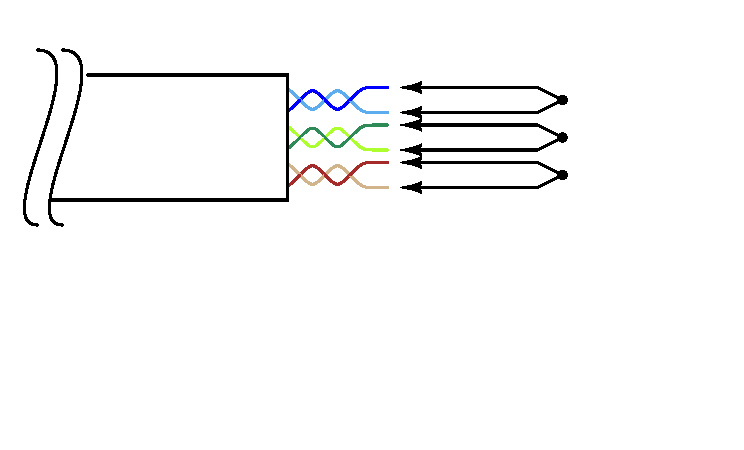
\includegraphics[scale=1,trim=0 1.5in 0 0]{hbusphys.ps}\\
   % translate x=1232 y=560 scale 0.38
   \putbox{4.06in}{2.72in}{1.20}{}%
   \putbox{1.64in}{0.06in}{1.20}{}%
   \putbox{4.56in}{0.97in}{1.20}{}%
   \putbox{3.72in}{0.72in}{1.20}{\midbox{RS485}}%
   \putbox{3.72in}{0.47in}{1.20}{\midbox{ALIMENTAÇÃO}}%
   \putbox{3.72in}{0.22in}{1.20}{\midbox{FREEBUS}}%
   } % close 'parbox'
   } % close 'scalebox'
   \vspace{-\baselineskip} % this is not necessary, but looks better
\end{center}

\caption{Cabo para transporte do barramento HBUS}
\end{figure}

No caso do uso de um cabo com 8 condutores, utiliza-se um par a mais para a alimentação. Note que o sinal FREEBUS não é diferencial. Ele vai trançado com um condutor ligado ao terra dos circuitos.

O conector também é padronizado para evitar complicações futuras. Os conectores e plugues utilizados são do tipo RJ-12, também conhecidos como 6P6C.

Recomenda-se fortemente que o dispositivo seja projetado com duas portas para conexão de cabos, abrindo a possibilidade de conectar muitos dispositivos em cadeia.

Uma observação muito importante é que por padrão os sinais \textbf{RS485} são conectados de forma cruzada, ou seja, o s sinais positivo e negativo são invertidos na conexão entre dois dispositivos, resultado numa conexão entre duas portas como a ilustrada abaixo:

\begin{figure}[H]
\centering
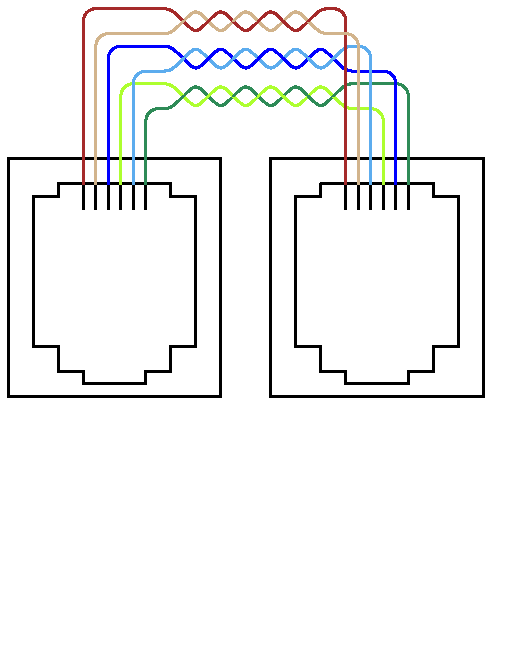
\includegraphics{../media/hbusinterconn.pdf}
\caption{Conexão entre duas portas}
\end{figure}

A recomendação anterior de que o dispositivo possua duas portas deve seguir a regra da conexão cruzada resultando num dispositivo que tem uma porta com o sinal RS485 invertido em relação a outra.

\section{RS485}

O barramento utiliza comunicação RS485 em half-duplex como mencionado. Uma topologia muito comum para drivers é mostrada na figura.

\begin{figure}[H]
\centering
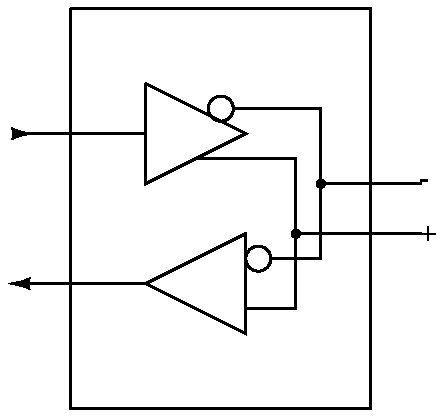
\includegraphics{../media/485drv.pdf}
\caption{Driver RS485}
\end{figure}

É recomendado o uso de um driver integrado deste tipo para a comunicação half-duplex. Há diversas opções de grandes fabricantes de semicondutores. No desenvolvimento foram usados drivers DS75176B.

\section{Alimentação}

A alimentação destinada aos dispositivos conectados ao barramento é de baixa potência devido a limitação imposta pelos condutores. O dispositivo deve ter o consumo mais econômico possível.

No caso de haver necessidade de uma maior potência, o dispositivo deve ser projetado para receber alimentação externa, sendo obrigatório o isolamento do barramento hbus através de soluções como os isoladores de RS-485 da Analog Devices.

Um outro caso é o uso de um repetidor de barramento. Isto é previsto e como é necessária a injeção de corrente, cai na mesma classificação do caso anterior.

Esta especificação não pretende definir limites extremamente rígidos para a tensão de alimentação no barramento, porém por questão de segurança todos os dispositivos devem suportar uma tensão mínima de 24 Volts.


\part{Software}

\chapter{A pilha de software HBUS}


Uma pilha de software que realiza as funções básicas de comunicação e controle é implementada. Este é um componente obrigatório para o dispositivo HBUS.

Esta pilha é composta por módulos que desempenham as funções:

\begin{itemize}

\item Definição de propriedades do dispositivo
\item Comunicação através do protocolo HBUS
\item Gerenciamento de interrupções
\item Gerenciamento do microcódigo HBUS

\end{itemize}

Neste capítulo é discutida a pilha como um todo e nos próximos são dados mais detalhes sobre os componentes da pilha.

Todo os dispositivos HBUS podem conter entradas e/ou saídas ou ainda variáveis internas que o desenvolvedor deseja que sejam acessíveis ao usuário através do barramento HBUS. Isto é realizado pela pilha, através de uma organização desses recursos em estruturas de dados que são manipuladas pela pilha.

Essas estruturas de dados são chamadas em geral de \textbf{Objetos}. São discutidas a seguir.

\newcommand{\tstrcommunication}{Protocolo de \\ Comunicação}
\newcommand{\tstrobjects}{Objetos}
\newcommand{\tstrucode}{Microcódigo}
\newcommand{\tstrhbusstack}{Pilha HBUS}
\newcommand{\tstrhbusdevice}{Dispositivo HBUS}
\newcommand{\tstrdevicecode}{Código do dispositivo (firmware)}

\begin{figure}[h]
\centering
\dtinput{../media/hbusdevice}
\caption{Arquitetura de software de um dispositivo HBUS}
\end{figure}

\section{Objetos de dispositivo}

Os objetos de dispositivo são estruturas de dados que encapsulam os dados a que o usuário do barramento HBUS terá acesso. Esses dados podem ser referentes a entradas, saídas ou outros valores específicos à programação de cada tipo de dispositivo.

Estes objetos são organizados por endereços. É possível ter até 255 objetos no dispositivo. A estrutura de dados que descreve um objeto é reproduzida a seguir.

\begin{minted}[linenos,bgcolor=bg]{c}

typedef struct HBUSOBJECTS
{
	HBUSOBJINFO objectInfo;
	
	byte * objectData;
	void * (*getObjectData)(void);
	void (*setObjectData)(void *, int);
	
} HBUSOBJ;

\end{minted}

Os campos da estrutura \textbf{HBUSOBJ} são detalhados na tabela a seguir.

\begin{table}[H]
\centering
\caption{Campos da estrutura HBUSOBJ}
\begin{tabular}{l p{12cm}}

\hline
Campo			&	Descrição\\
\hline
objectInfo		&	Estrutura contendo informações sobre o objeto. É detalhada mais adiante\\
objectData		&	Ponteiro para localização na memória que contem o valor referente ao objeto\\
getObjectData	&	Ponteiro para função que realiza leitura do valor do objeto\\
setObjectData	&	Ponteiro para função que realiza escrita do valor do objeto\\
\hline

\end{tabular}
\end{table}

Os dados referentes ao objeto podem ser acessados de duas maneiras:

\begin{enumerate}

\item O objeto fornece o campo objectData e a leitura e escrita são realizadas diretamente na memória.
\item O objeto fornece os campos get/setObjectData e a leitura e escrita são realizadas através das funções disponibilizadas pelo desenvolvedor para isso.

\end{enumerate}

Em outras palavras, o desenvolvedor tem a possibilidade de escolha se o valor a ser lido/escrito é um valor residente na memória ou se são usadas funções para realizar a tarefa. Note que a utilização de funções permite ao desenvolvedor saber que o objeto está sendo lido ou escrito no momento em que aquela função é chamada. Isto é muito útil em casos em que o valor só está disponível para ser transmitido após algum tipo de processamento.

Seguindo a filosofia de alocação de recursos, não faz sentido calcular constantemente este valor apenas para que no caso de ser requisitado ao dispositivo que envie-o, ele estar disponível. Utilizando-se de funções, o valor pode ser calculado sob demanda e imediatamente submetido.

\vskip1cm

A seguir é mostrada e analisada a estrutura contida no campo \textit{objectInf}o, que descreve as propriedades do objeto.

\pagebreak

\begin{minted}[linenos,bgcolor=bg]{c}

typedef struct HBUSOBJECTINFOS
{
	byte objectFlags;
	byte objectSize;
	
	byte objectDataTypeInfo;
	
	byte objectDescStringSize;
	byte * objectDescString;
	
} HBUSOBJINFO;

\end{minted}

Os campos e possíveis flags são analisados nas tabelas a seguir.

\begin{table}[H]
\centering
\caption{Campos da estrutura HBUSOBJINFO}
\begin{tabular}{l p{10cm}}

\hline
Campo					&	Descrição\\
\hline
objectFlags				&	Byte contendo flags do objeto\\
objectSize				&	Tamanho do objeto em bytes\\
objectDataTypeInfo		&	Informações secundárias sobre a interpretação do tipo de dados do objeto\\
objetcDescStringSize		&	Tamanho da string descritiva do objeto em bytes\\
objectDescString			&	Ponteiro para a string descritiva\\
\hline

\end{tabular}
\end{table}

\begin{table}[H]
\centering
\caption{Possíveis flags para o objeto}
\begin{tabular}{l c l}

\hline
Flag						& 	Valor	&	Descrição\\
\hline
HBUSOBJ\_READ			&	0x01		&	O barramento tem permissão de leitura do objeto\\
HBUSOBJ\_WRITE			&	0x02		&	O barramento tem permissão de escrita no objeto\\
HBUSOBJ\_CRYPTO			&   0x04	    &	Dados do objeto são trafegados criptografados\\
HBUSOBJ\_HIDDEN			&	0x08		&	Este objeto não é visível para o usuário\\
\hline

\end{tabular}
\end{table}

Esses objetos são declarados no arquivo \textit{hbus\_objects.c}. Eles devem ser declarados como do tipo \textbf{const}, para que sejam alocados na memória de programa, já que são informações imutáveis em tempo de execução, liberando assim memória RAM para alocação de variáveis mais importantes.

Os objetos são indexados pela variável \textbf{MCU\_OBJECTS[]}, sendo que o primeiro objeto, com endereço 0 é um objeto obrigatório especial que contem informações sobre o dispositivo. Os objetos implementados pelo desenvolvedor são alocados a partir do índice 1.

\subsection{Os objetos especiais}

São definidos alguns tipos de objetos de dispositivo especiais. É um requerimento obrigatório o suporte a estes objetos. Todos os dispositivos devem suportá-los.

\subsubsection*{O objeto zero}

O objeto de endereço 0 é especial e contem uma estrutura de dados específica que descreve o dispositivo. Além disso, a string descritiva deste objeto deve ser o nome do dispositivo e este objeto é somente para leitura.

O campo \textit{objectData} deve apontar para uma estrutura do tipo \textbf{HBUSOBJLISTINFO}. Esta estrutura é mostrada a seguir.

\begin{minted}[linenos,bgcolor=bg]{c}

typedef struct HBUSOBJECTLISTINFOS
{
	byte objectListSize;
	byte endpointListSize;
	byte interruptListSize;
	
	byte slaveCapabilities;
	
	dword uniqueDeviceInfo;
	
} HBUSOBJLISTINFO;

\end{minted}

\begin{table}[H]
\centering
\caption{Campos da estrutura HBUSOBJLISTINFO}
\begin{tabular}{l p{13cm}}

\hline
Campo					&	Descrição\\
\hline
objectListSize			&	Tamanho da lista de objetos do dispositivo (quantidade de objetos)\\
endpointListSize			&	Tamanho da lista de endpoints do dispositivo\\
interruptListSize		&	Tamanho da lista de interrupções do dispositivo\\
slaveCapabilities		&	Funções opcionais habilitadas no dispositivo\\
uniqueDeviceInfo			&	Valor de identificação único do dispositivo (4 bytes)\\
\hline

\end{tabular}
\end{table}

Em especial, o campo \textit{uniqueDeviceInfo} deve ser observado. Neste campo é obrigatório colocar um identificador único do dispositivo, como uma espécie de número serial. A recomendação padrão é usar metade do campo para criar um identificador de família do objeto e a outra metade um número serial.

Além disso, a partir da versão 1.1, existe o campo \textit{slaveCapabilities}, que contém informações sobre as funções opcionais HBUS (microcódigo, interrupções, endpoints, criptografia e autenticação) habilitadas no dispositivo em questão.

\begin{table}[H]
\centering
\caption{Flags no campo \textit{slaveCapabilities}}
\begin{tabular}{c p{13cm}}
\hline
ID		&	Significado\\
\hline
0x01		&	Dispositivo tem suporte a criptografia (privacidade de objetos)\\
0x02		&	Dispositivo tem suporte a endpoints\\
0x04		&	Dispositivo tem suporte a emissão de interrupções\\
0x08		&	Dispositivo tem suporte a autenticação do mestre\\
0x10		&	Dispositivo tem suporte a microcódigo\\
0x20		&	Dispositivo tem suporte a autenticação reversa (autenticação de dispositivo)\\
\hline
\end{tabular}
\end{table}

\subsubsection*{O objeto de broadcast de informações}

Este objeto é na verdade um objeto emulado no número 255 para todos os dispositivos. Não é necessário realizar a declaração deste objeto. No entanto, a máquina de estados do dispositivo deve estar apta a receber dados através deste objeto e é necessário observar alguns detalhes importantes.

O objeto de broadcast existe para que o mestre possa enviar informações periódicas e alertas ao sistema como um todo. Dessa forma, é possível, com uma mensagem apenas, informar todos os dispositivos de alguma condição de alerta no barramento ou realizar sincronização periódica, por exemplo. Este tipo de objeto é somente para escrita.

A transferência de informações é realizada através de um comando \hbuscommand{SETCH} no objeto 255, realizado para todos os dispositivos de um barramento ao mesmo tempo (utilizando o endereço de broadcast). A informação transmitida é identificada por uma subclasse através dos dois primeiros bytes transmitidos na operação. As 128 primeiras subclasses são reservadas ao mestre HBUS e as restantes podem ser implementadas por terceiros.


\subsection{Os tipos de dados de objetos}

Os tipos de dados auxiliam o mestre na interpretação dos dados obtidos dos dispositivos. Há duas informações principais para cada objeto do dispositivo: o tipo de dado propriamente dito e uma informação secundária sobre a formatação deste dado.

A informação sobre o tipo de dado que deve ser associado ao objeto na interpretação do mesmo é colocado junto aos flags do objeto no campo \textit{objectFlags}.

\begin{table}[H]
\centering
\label{table:datatypes}
\caption{Flags para o tipo de dados do objeto}
\begin{tabular}{l c l}
\hline
Flag					&	Valor	& Tipo de dado\\
\hline
HBUSOBJ\_DTYPE\_INT	&	0x10		& Inteiro\\
HBUSOBJ\_DTYPE\_UINT	&	0x20		& Inteiro sem sinal\\
HBUSOBJ\_DTYPE\_FIXP	&	0x40		& Ponto Fixo\\
HBUSOBJ\_DTYPE\_BYTE	&	0x80		& Vetor de bytes\\
\hline
\end{tabular}
\end{table}

As informações secundárias estão contidas no campo \textit{objectDataTypeInfo}. As opções variam de acordo com os tipos de dados especificados na tabela \ref{table:datatypes} e são discutidas a seguir:

\subsubsection*{O tipo de dados Inteiro}

Os objetos que utilizam este tipo de dados terão seus valores interpretados como sendo inteiros de tamanho padrão (4 bytes). Assim, 4 bytes é o tamanho máximo para estes objetos.

Este tipo de dados não possui opções de formatação definidas.

\subsubsection*{O tipo de dados Inteiro sem sinal}

Os objetos do tipo inteiro sem sinal são tratados como tal. O tamanho máximo é 4 bytes.

Suas possíveis opções de formatação para auxiliar a interpretação:


\begin{table}[H]
\centering
\caption{Formatação dos objetos do tipo inteiro sem sinal}
\scalebox{0.75}{
\begin{tabular}{l c p{10cm}}
\hline
ID								&	Valor	&	Descrição\\
\hline
HBUSOBJ\_DTYPE\_UINT\_PERCENT		&	0x04		&	O dado é um valor percentual (0-100)\\
HBUSOBJ\_DTYPE\_UINT\_LIN\_PERCENT	&	0x05		&	O dado é um inteiro sem sinal que deverá ser interpretado como um percentual em uma escala linear\\
HBUSOBJ\_DTYPE\_UINT\_LOG\_PERCENT	&	0x06		&	O dado é um inteiro sem sinal que deverá ser interpretado como um percentual em uma escala logarítmica\\
HBUSOBJ\_DTYPE\_UINT\_TIME			&	0x09		&	O dado é um valor temporal no padrão HBUS\\
HBUSOBJ\_DTYPE\_UINT\_DATE			&	0x0A		&	O dado é um valor de data no padrão HBUS\\
\hline
\end{tabular}
}
\end{table}


\subsubsection*{O tipo de dados Ponto Fixo}

Estes objetos deverão ser tratados como inteiros com sinal, porém são fracionários em sua natureza e a localização do ponto decimal é dada pelo valor do campo \textit{objectDataTypeInfo}.

\subsubsection*{O tipo de dados Vetor de bytes}

Estes objetos não possuem tamanho máximo. São interpretados como uma sequência de bytes (os bytes são equivalentes a um número inteiro menor ou igual a 255, sem sinal).

\begin{table}[H]
\centering
\caption{Formatação dos objetos do tipo vetor de bytes}
\scalebox{0.75}{
\begin{tabular}{l c p{10cm}}
\hline
ID								&	Valor	&	Descrição\\
\hline
HBUSOBJ\_DTYPE\_BYTE\_BASE\_HEX		&	0x01		&	O dado é exibido na base hexadecimal\\
HBUSOBJ\_DTYPE\_BYTE\_BASE\_DEC		&	0x02		&	O dado é exibido na base decimal\\
HBUSOBJ\_DTYPE\_BYTE\_BASE\_OCT		&	0x03		&	O dado é exibido na base octal\\
HBUSOBJ\_DTYPE\_BYTE\_BASE\_BIN		&	0x07		&	O dado é exibido na base binária\\
HBUSOBJ\_DTYPE\_BYTE\_STRING			&	0x0B		&	O dado é exibido como sendo um vetor de caracteres ASCII\\
\hline
\end{tabular}
}
\end{table}

\subsection{Os objetos invisíveis}
\label{sec:hiddenobj}

Os objetos invisíveis são um novo conceito introduzido na versão 1.1.1. Estes objetos não são visíveis ao usuário do barramento HBUS. No entanto, podem ser usados para trocar informações importantes entre os escravos e o mestre.

Estes objetos não devem conter informações sobre tipos de dados nem também um nome próprio. Podem ser usados para transferência de informações extendidas sobre os objetos como limites de valores ou outras informações extendidas. Todos os objetos invisíveis são relativos a um dos outros objetos do dispositivo.

\subsubsection*{A sintaxe dos objetos invisíveis}

A sintaxe para interpretação dos objetos invisíveis é utilizada no campo de descrição do objeto e é extremamente simples:

\begin{equation*}
n:CAMPO
\end{equation*}

Onde \textit{n} é o número do objeto a que este outro objeto se refere e \textit{CAMPO} é o campo associado. Os campos padrão definidos pela especificação HBUS são:

\begin{table}[H]
\centering
\begin{tabular}{l l}
\hline
Campo		&		Uso\\
\hline
MIN			&		Especifica valor mínimo possível do objeto\\
MAX			&		Especifica valor máximo possível do objeto\\
UNIT			&		Especifica uma unidade de medida para o valor do objeto\\
STR			&		Associa um texto ao objeto\\
USR			&		Dados genéricos do usuário\\
PUBKEY		&		Chave pública do dispositivo quando presente. Deve ser associado ao objeto 0\\
\hline
\end{tabular}
\caption{Campos para objetos invisíveis}
\end{table}

Os valores que serão associados ao objeto referido são os valores contidos no objeto invisível declarado para tal fim.

\subsubsection*{Exemplos de utilização}

Seja um objeto que implementa a escrita e leitura de um valor X, que é um inteiro sem sinal sem formatação específica. Assuma que este é o objeto número 1 do dispositivo:

\begin{minted}[linenos,bgcolor=bg]{c}

const HBUSOBJ VALOR_X = {{HBUSOBJ_WRITE|HBUSOBJ_READ|HBUSOBJ_DTYPE_UINT,2,
			0x00,12,"VALOR X"},0x00,LE_X,ESCREVE_X};

\end{minted}

Imagine que se queira atribuir uma faixa de valores válidos para este objeto, em outras palavras um valor máximo e um mínimo. Dois objetos invisíveis podem solucionar o problema:

\begin{minted}[linenos,fontsize=\small,bgcolor=bg]{c}

const word VALOR_MINIMO = 0x0010;
const word VALOR_MAXIMO = 0xF000;

const HBUSOBJ VALOR_X_MIN = {{HBUSOBJ_READ|HBUSOBJ_HIDDEN,2,0x00,12,"1:MIN"},
				(byte*)&VALOR_MINIMO,0x00,0x00};
								
const HBUSOBJ VALOR_X_MAX = {{HBUSOBJ_READ|HBUSOBJ_HIDDEN,2,0x00,12,"1:MAX"},
				(byte*)&VALOR_MAXIMO,0x00,0x00};

\end{minted}

Isto indicará com sucesso ao mestre como interpretar os dados e quais são valores válidos para escrita e leitura do objeto.

\section{Endpoints de dispositivo}

Os endpoints são um tipo especial de objeto que tem uma forma de acesso diferenciada. Eles são indexados em um espaço de endereçamento diferente dos objetos de dispositivo. O uso de endpoints é opcional e inclusive é possível compilar a pilha HBUS sem suporte a endpoints se for necessário por questões de economia de espaço.

A função de um endpoint é realizar a leitura ou escrita de um grande volume de bytes em uma única transmissão.

Sua implementação é muito parecida com a dos objetos de dispositivo. A estrutura de dados que define um endpoint é mostrada a seguir:

\begin{minted}[linenos,bgcolor=bg]{c}

typedef struct HBUSENDPOINTS
{
	HBUSEPINFO endpointInfo;
	
	byte * dataStart;
	
	byte (*readEPByte)(void);
	byte (*writeEPByte)(byte);
	
	void (*EPwriteBegin)(void);
	void (*EPwriteEnd)(void);
	
	void (*EPreadBegin)(void);
	void (*EPreadEnd)(void);
	
} HBUSEP;

\end{minted}

\begin{table}[H]
\centering
\caption{Campos da estrutura HBUSEP}
\begin{tabular}{l p{12cm}}

\hline
Campo					&	Descrição\\
\hline
endpointInfo				&	Estrutura contendo informações sobre o endpoint\\
dataStart				&	Ponteiro para localização na memória do início dos dados\\
readEPByte				&	Ponteiro para uma função que escreve um byte na memória do endpoint\\
writeEPByte				&	Ponteiro para uma função que lê um byte da memória do endpoint\\
EPwriteBegin				&	Ponteiro para uma função que é chamada assim que começa a escrita do endpoint\\
EPwriteEnd				&	Ponteiro para uma função que é chamada assim que termina a escrita do endpoint\\
EPreadBegin				&	Ponteiro para uma função que é chamada assim que começa a leitura do endpoint\\
EPreadEnd				&	Ponteiro para uma função que é chamada assim que termina a leitura do endpoint\\
\hline

\end{tabular}
\end{table}

De maneira análoga a implementação de objetos do dispositivo, os campos dataStart e readEPByte e writeEPByte são intercambiáveis.

Todas os demais ponteiros para funções são opcionais. Seguindo a análise, será vista a estrutura \textbf{HBUSEPINFO}.

\begin{minted}[linenos,bgcolor=bg]{c}

typedef struct HBUSENDPOINTINFOS
{
	byte endpointFlags;
	byte endpointBlockSize;
	
	byte endpointDescStringSize;
	byte * endpointDescString;
	
} HBUSEPINFO;

\end{minted}

Mais uma vez a implementação é análoga a de objetos de dispositivo. A maior diferença nesse caso é o campo \textit{endpointBlockSize}, que descreve o tamanho do bloco de dados que é representado no barramento HBUS pelo endpoint.

\section{Interrupções de dispositivo}

As interrupções também são descritas por um tipo especial de objeto que assim como no caso dos endpoints, são endereçados e acessados de forma diferente dos objetos comuns. Todos os objetos de interrupção são por definição somente de leitura, uma vez que sua única funcionalidade é descrever uma interrupção que o dispositivo pode vir a disparar no barramento.

Os objetos de interrupção são definidos pelas estruturas mostradas:

\begin{minted}[linenos,bgcolor=bg]{c}

typedef struct HBUSINTERRUPTINFOS
{
	byte interruptFlags;
	
	byte interruptDescStringSize;
	byte * interruptDescString;
	
} HBUSINTINFO;

typedef struct HBUSINTERRUPTS
{
	
	HBUSINTINFO interruptInfo;
	
	byte interruptNumber;
	
} HBUSINT;

\end{minted}

Mais uma vez a implementação é claramente análoga a dos objetos de dispositivo. Observações:


\begin{itemize}

\item Cada interrupção possui um número de identificação.
\item Os flags da interrupção não foram implementados até o momento
\item A emissão de interrupções e seu código na pilha HBUS é opcional e a sua compilação pode ser desativada. No entanto, a monitoração do sinal FREEBUS é obrigatória.

\end{itemize}

\section{Objetos especiais do mestre}

Os objetos especiais do mestre são objetos requeridos que contém dados como data/hora e outros.

Como não é permitido aos dispositivos iniciarem comunicações que não são interrupções, a leitura destes objetos especiais é feita da seguinte maneira:

\begin{enumerate}
\item O dispositivo envia uma interrupção do tipo \textbf{INFOREQUEST} ao mestre.
\item O mestre responde com um comando do tipo \hbuscommand{ACK}, informando ao dispositivo que o pedido de informações foi aceito
\item O mestre realiza um \hbuscommand{BUSLOCK} com o dispositivo.
\item O dispositivo, usando o barramento travado, executa um comando \hbuscommand{GETCH} para ler o objeto especial do mestre.
\end{enumerate}



\section{O ciclo e inicialização da pilha HBUS}

A pilha HBUS é inicializada no RESET do dispositivo hóspede e ciclos são executados repetidamente durante toda o tempo de execução.

\begin{figure}[H]
\centering
\dtinput{../media/hbusstack}
\caption{Funcionamento da pilha HBUS}
\end{figure}


\chapter{O protocolo de comunicação HBUS}



A especificação HBUS define um protocolo de comunicação ponto-a-ponto. Este protocolo é explorado em detalhes neste capítulo.

\section{Estrutura de uma mensagem HBUS}

Os quadros de mensagem HBUS são constituídos de vários campos, onde se identificam os dispositivos fonte e destino da mensagem, além do conteúdo da mensagem.

\subsection{Alocação de endereços para os dispositivos}

Será usado a partir de agora o conceito de barramento local e barramento global. A especificação HBUS permite um ou mais barramento HBUS seja conectado a outro barramento por meio de um repetidor. Isto é feito para aumentar a capacidade de conexão de dispositivos no sistema como um todo. Note que ainda continuará existindo apenas um mestre. A ação da repetição do barramento gera um novo barramento com endereço diferente do originário. O barramento global é o sistema composto por todos os dispositivos HBUS conectados a todos os sub barramentos interconectados.

Cada dispositivo no barramento global possui um endereço. Este endereço é composto por dois bytes, sendo um referente ao número do barramento local no qual o dispositivo está conectado e o outro é o endereço do dispositivo dentro deste barramento.

\subsection{O pacote HBUS}

De forma geral as transmissões são realizadas em pacotes que seguem o esquema mostrado na figura a seguir. Na figura, cada quadrado representa um byte transmitido.

\newcommand{\SDSTR}{Endereço do \\ disp. fonte}
\newcommand{\TDSTR}{Endereço do \\ disp. alvo}
\newcommand{\CMDSTR}{Comando}
\newcommand{\TERMSTR}{Fim}
\newcommand{\DATASTR}{Dados}
\newcommand{\ADDRSTR}{Endereço}
\newcommand{\SIZESTR}{Tamanho}

\begin{figure}[H]
\centering
\dtinput{../media/hbuspacket}
%\import{../media/}{hbuspacket}
\caption{Pacote HBUS}
\end{figure}

Dependendo do comando, a seção de dados do pacote pode conter um número diferente de bytes. Para alguns comandos este número pode ser inclusive zero.

O byte terminador tem valor obrigatório de 0xFF.

\section{Os comandos HBUS}

O conjunto de comandos padrão do barramento HBUS é discutido. A tabela mostra a lista de comando disponíveis.

\begin{table}[H]
\centering
\caption{Comandos HBUS}
\begin{tabular}{c c p{4cm} p{6cm}}
\hline
Comando	 &	 Código 		&	Parâmetros				&	 Descrição\\
\hline
SETCH	&	0x01			&	Endereço	 do objeto e tamanho em bytes		&	Escreve no objeto do dispositivo se o mesmo tem permissão de escrita\\
GETCH	&	0x04			&	Endereço do objeto		&	Lê objeto do dispositivo caso tenha permissão de leitura\\
RESPONSE&	0x10			&	Endereço do objeto origem e tamanho em bytes & Envia o valor do objeto que foi requisitado pelo comando GETCH\\
SEARCH	&	0x03			&	---						&	Inicia o processo de endereçamento dos dispositivos ou verifica presença de um dispositivo já endereçado\\
ACK		&	0x06			&	---						&	Comando para indicar que mestre ou dispositivo confirmaram algum processo anterior.\\
ERROR	&	0x20			&	Código de erro			&	Comando para retorno de códigos de erro. Opcional.\\
QUERY	&	0x07		&	Endereço do objeto		&	Lê informações sobre o objeto. O dispositivo envia a estrutura HBUSOBJINFO.\\
QUERY\_EP &	0x11		&	Endereço do endpoint		&	Análogo ao comando QUERY, porém voltado aos endpoints.\\
QUERY\_INT&	0x12		&	Endereço da interrupção	&	Funcionamento similar aos dois comandos anteriores.\\
QUERY\_RESP & 0x08		&	Endereço do objeto origem & As informações do objeto, endpoints e interrupções são retornadas através deste comando.\\
STREAMW	&	0x40			&	Endereço do endpoint e tamanho do bloco		&	Realiza escrita no endpoint selecionado se houver permissão.\\
STREAMR	&	0x41			&	Endereço do endpoint		&	Realiza leitura no endpoint.\\
BUSLOCK	&	0xF0			&	---						& 	Causa o travamento exclusivo do barramento para comunicações entre os dois dispositivos envolvidos na mensagem.\\
BUSUNLOCK&	0xF1			&	---						&	Finaliza o travamento exclusivo do barramento, liberando-o.\\
SOFTRESET&	0xF2			&	---						&	Ocasiona um RESET por software no dispositivo.\\
KEYSET	&	0xA0			&	Chave pública do mestre	&	Registra chave pública do mestre no dispositivo.\\
KEYRESET	&	0xA1			&	Bloco de assinatura		&	Remove registro de chave pública do dispositivo.\\
\hline
\end{tabular}
\end{table}

A seguir uma análise mais detalhada é feita.

\subsection{Os comandos SETCH, GETCH e RESPONSE}

Esses três comandos estão envolvidos com a tarefa de escrita e leitura em objetos do dispositivo.

\subsubsection{SETCH}

O comando \hbuscommand{SETCH} realiza a escrita em um objeto do dispositivo. O dispositivo deve, após aceitar o comando, verificar se o objeto possui permissão de escrita. Caso possua, o novo valor enviado é escrito no objeto. Caso contrário o dispositivo pode enviar de volta uma mensagem utilizando o comando \hbuscommand{ERROR} ou não enviar nada.

Os parâmetros do comando \hbuscommand{SETCH} são o endereço do objeto no dispositivo e o tamanho em bytes a ser escrito. A figura \ref{fig:setch} mostra a estrutura de uma mensagem usando o comando \hbuscommand{SETCH}. Não é mostrada a parte inicial de endereçamento para simplicidade.

\begin{figure}[H]
\centering
\dtinput{../media/setch}
\caption{O comando \hbuscommand{SETCH}}
\label{fig:setch}
\end{figure}

\subsubsection{GETCH}

Este comando realiza a leitura de um objeto do dispositivo. Após aceitar o comando, se o objeto tem permissão de leitura, o dispo sito enviará um comando \hbuscommand{RESPONSE} contendo os dados do objeto. Caso contrário pode enviar ou não uma mensagem com o comando \hbuscommand{ERROR}.

\begin{figure}[H]
\centering
\dtinput{../media/getch}
\caption{O comando \hbuscommand{GETCH}}
\end{figure}

\subsubsection{RESPONSE}

Após a utilização do comando \hbuscommand{GETCH}, o dispositivo deve retornar a informação através do comando \hbuscommand{RESPONSE}.
A estrutura parcial da mensagem é vista a seguir.

\begin{figure}[H]
\centering
\dtinput{../media/response}
\caption{O comando \hbuscommand{RESPONSE}}
\end{figure}

\subsection{Os comandos QUERY, QUERY\_EP, QUERY\_INT e QUERY\_RESP}

Estes comandos são relacionados a obtenção de informações sobre os objetos de dispositivo e suas variações: endpoints e interrupções. O mestre não precisa ter conhecimento prévio sobre um dispositivo qualquer que é conectado ao barramento. Através deste mecanismo, ele pode obter todas as informações através do próprio barramento.

Os comandos \hbuscommand{QUERY}, \hbuscommand{QUERY\_EP} e \hbuscommand{QUERY\_INT} buscam informações dos objetos de dispositivo, endpoints e interrupções, respectivamente.

\begin{figure}[H]
\centering
\dtinput{../media/query}
\caption{Os comandos \hbuscommand{QUERY}}
\end{figure}

O comando \hbuscommand{QUERY\_RESP} é enviado pelo dispositivo em resposta a recepção de um comando tipo \hbuscommand{QUERY($\cdots$)}. Junto a este comando é enviada a estrutura do tipo \textbf{HBUSOBJINFO}, \textbf{HBUSEPINFO} ou \textbf{HBUSINTINFO} correspondente ao objeto no dispositivo.

\begin{figure}[H]
\centering
\dtinput{../media/query_resp}
\caption{O comando \hbuscommand{QUERY\_RESP}}
\end{figure}

\subsection{Os comandos STREAMW e STREAMR}

Estes comandos tem como finalidade o início de escrita e leitura de um bloco de bytes em um dos endpoints do dispositivo. Seu funcionamento é descrito a seguir.

\subsection{Os comandos BUSLOCK e BUSUNLOCK}

Utilizados como peça chave em algumas operações do barramento, além de poderem ser usados livremente pelo mestre, esses comandos tem como finalidade o travamento exclusivo do barramento para tráfego de dados entre dois dispositivos.

Todos os dispositivos escutam o barramento constantemente. Ao detectar a emissão de um comando \hbuscommand{BUSLOCK} no barramento, o dispositivo deve verificar se aquele comando é endereçado a ele. Caso seja, ele aceitará as transmissões posteriores. Caso contrário, deve ignorar todas as transmissões até que seja emitido no barramento o comando \hbuscommand{BUSUNLOCK}.

É uma definição obrigatória que o período máximo de duração de um \hbuscommand{BUSLOCK} é de 1 minuto. Se esse tempo for atingido sem a emissão de um comando \hbuscommand{BUSUNLOCK}, os dispositivos devem automaticamente sair do estado travado e aceitar transmissões.

\subsection{O comando SEARCH}

O comando \hbuscommand{SEARCH} é utilizado para duas finalidades diferentes:

\begin{enumerate}

\item Utilizado no processo de endereçamento dos dispositivos;
\item Utilizado para monitorar a presença de um dispositivo já endereçado no barramento. Este procedimento é simples e tem dois passos:
\begin{enumerate}
\item O mestre envia o comando \hbuscommand{SEARCH}.
\item O dispositivo, se ainda está presente no barramento, é obrigado a enviar o comando \hbuscommand{ACK}.
\item O mestre aguarda. Se receber o comando \hbuscommand{ACK}, sabe que o dispositivo está ativo. Se se passar um tempo especificado e não for recebido o comando, sabe-se que o dispositivo se desconectou do barramento.
\end{enumerate}

\end{enumerate}

\subsubsection{Recomendação de implementação}

É recomendado que o mestre monitore o barramento com uma frequência dependente da natureza da rede implantada utilizando-se do barramento HBUS. Na grande maioria das vezes a rede é fixa e não sofre mudanças, de forma que geralmente esse monitoramento ocorrerá em um período relaxado.

As principais razões para realizar o monitoramento periódico da rede com o comando \hbuscommand{SEARCH} são óbvias:
detecção de novos dispositivos e detecção da desconexão (ou falha) de dispositivos.

\subsection{Os comandos ACK e ERROR}

Os comandos \hbuscommand{ACK} e \hbuscommand{ERROR} servem para enviar respostas positivas e negativas, respectivamente, ao mestre. São usados em situações específicas descritas neste documento.

\subsection{O comando INT}

O comando \hbuscommand{INT} é enviado pelo dispositivo no processo de interrupção. Este processo é discutido num capítulo próximo.

\subsection{O comando SOFTRESET}

Este comando, quando recebido pelo dispositivo, requer que o mesmo execute um reset por software nele mesmo.
Na plataforma utilizada para o desenvolvimento, isto é alcançado realizando-se a execução proposital de uma instrução ilegal.

\subsection{Os comandos KEYSET E KEYRESET}

Presentes a partir da versão 1.1, estes comandos são reconhecidos apenas por dispositivos que possuem suporte a autenticação de mestre.

\subsubsection{KEYSET}

O comando \hbuscommand{KEYSET} é executado no processo de endereçamento apenas no caso de o dispositivo em questão suportar a autenticação de mestre. Através deste comando é informada ao dispositivo a chave pública do mestre, utilizada para assinar as mensagens de escrita e garantir a autenticidade das mesmas.

Este comando somente grava uma nova chave no dispositivo caso o mesmo não tenha sido previamente associado a nenhum mestre. Neste caso, ao receber o comando, o dispositivo automaticamente grava de forma permanente a chave e torna-se associado ao mestre que enviou o comando. A única maneira de o dispositivo ser desassociado deste mestre é a emissão de um comando \hbuscommand{KEYRESET}, assinado corretamente.

Caso o dispositivo já esteja associado a um mestre e receber o comando \hbuscommand{KEYSET} no processo de endereçamento, o dispositivo compara a chave recebida com a sua chave previamente gravada e duas situações são possíveis:

\begin{enumerate}

\item As chaves são iguais e o dispositivo está sendo endereçado pelo mestre correto. O dispositivo entra em operação normal.

\item As chaves são diferentes e o dispositivo está sendo endereçado por um outro mestre. Neste caso o dispositivo tem a escolha de recusar o endereçamento ou entrar em modo de operação somente leitura.

\end{enumerate}

\subsubsection{KEYRESET}

Este comando realiza a desassociação do dispositivo com o mestre. É necessário que este comando contenha uma assinatura válida.

Esta ação libera o dispositivo para ser utilizado em outros barramentos, com outro mestre.

\section{O processo de endereçamento do dispositivo}

Todos os dispositivos, quando conectados ao barramento, necessitam esperar que o mestre realize o processo de endereçamento. Mais uma vez é seguida a filosofia de não-ocupação do canal.

O dispositivo, na sua inicialização assume o endereço 255 no barramento. Este é um endereço especial reservado.

\subsection{O endereço de broadcast}

O endereço reservado 255 é chamado de endereço de broadcast, porque todos os dispositivos ainda não-endereçados são obrigados a escutar o barramento neste endereço e obedecer quaisquer mensagens que sejam direcionadas ao endereço de broadcast.

É através deste endereço, que é iniciado o processo de endereçamento do dispositivo.

\subsection{Endereçamento passo a passo}

Uma descrição passo a passo do processo de endereçamento do dispositivo:

\begin{enumerate}

\item O dispositivo completa sua inicialização e aguarda, escutando o barramento no endereço 255.
\item O mestre dá início ao processo de endereçamento através do envio de um comando \textbf{SEARCH} para o endereço de broadcast.
\item O dispositivo aguarda um período de guarda de alguns milissegundos que é definido aleatoriamente. A razão para isto é discutida em seguida.
\item Após passado o período de guarda, o dispositivo envia um comando \hbuscommand{BUSLOCK} para o mestre. O barramento está então travado. O dispositivo aguarda o mestre.
\item O mestre deve enviar um comando \hbuscommand{GETCH}, requisitando o objeto 0 do dispositivo, para obter suas funcionalidades.
\item O dispositivo envia o conteúdo do objeto 0 ao mestre.
\item Se o dispositivo tem suporte a autenticação, o mestre envia o comando \hbuscommand{KEYSET}, acompanhado da sua chave pública, endereçado ao endereço que será atribuído.
\item Caso o dispositivo não possua suporte a autenticação, o mestre envia novamente o comando \hbuscommand{SEARCH}, porém desta vez para o endereço que será atribuído ao dispositivo.
\item O dispositivo recebe o comando e assume o endereço contido no pacote.
\item O dispositivo envia o comando \hbuscommand{BUSUNLOCK} e o barramento é destravado. Chega ao fim o processo de endereçamento.

\end{enumerate}

\subsection{Prevenção de colisões no endereçamento}

Quando um barramento desenergizado com vários dispositivos já conectados é alimentado, todos os dispositivos estão no estado não-endereçado. Quando o mestre emitir o comando \hbuscommand{SEARCH}, é preciso que haja algum esquema para impedir a colisão de dispositivos que tem inicialmente o mesmo endereço (broadcast) ao tentar realizar o endereçamento.

Para isso é estabelecido o período de guarda aleatório mencionado anteriormente. Sendo o período aleatório, fatalmente um dispositivo irá travar o barramento antes dos demais, garantindo que só ele está realizando o processo de endereçamento nesta etapa, uma vez que os outros dispositivos, sabendo do estado ocupado do barramento não podem tentar realizar transmissões.

Quando o barramento estiver livre novamente, os outros dispositivos podem iniciar seu processo de endereçamento, aplicando sempre o período de guarda aleatório. Dessa maneira, os dispositivos vão completando o processo de endereçamento sucessivamente até que todos estejam endereçados no barramento.

\subsection{Recomendações}

É recomendado que assim que o processo de endereçamento for terminado, o mestre realize a identificação dos objetos através dos comandos \hbuscommand{QUERY}, obtendo assim informações sobre todos os objetos de todos os dispositivos conectados. Essas informações devem ser guardadas para facilitar o acesso aos dispositivos durante a execução.

\section{O acesso aos objetos do tipo endpoint}

O acesso a estes objetos é feito através dos comandos \hbuscommand{STREAMW} e \hbuscommand{STREAMR}. No entanto, estes comandos apenas iniciam o processo de acesso, que é feito em algumas etapas:

\begin{enumerate}

\item O mestre envia um comando \hbuscommand{STREAMW} ou \hbuscommand{STREAMR} ao dispositivo.
\item O dispositivo recebe o comando e se as permissões do endpoints forem coerentes com o comando recebido, o dispositivo executa um comando \hbuscommand{BUSLOCK}, travando o uso do barramento entre ele e o mestre.
\item No ato da recepção do \textbf{BUSLOCK}, o mestre assume que a transmissão será realizada. No caso de uma transmissão de escrita, o mestre envia os dados ao barramento travado, não sendo nenhum tipo de formatação requerida.
No caso de uma transmissão de leitura, o escravo, após executar o \hbuscommand{BUSLOCK}, começa a enviar imediatamente os dados.
\item Após a transmissão ser concluída, o escravo emite o comando \hbuscommand{BUSUNLOCK}, liberando o barramento para as comunicações.

\end{enumerate}

\subsection{A importância e expansibilidade dos endpoints}

Pode não ser aparente a primeira vista, porém o sistema de endpoints tem uma importância chave.

Devido a natureza da transmissão, que é realizada sobre o barramento travado exclusivamente para os dois dispositivos envolvidos e ainda o detalhe que durante a transmissão, os dispositivos não processam os dados da forma usual mostrada até agora, deixa-se aberta a possibilidade de implementação de protocolo secundários sobre o protocolo de comunicação HBUS através do uso de endpoints.

Esses protocolos secundários podem ser muito importantes para o dispositivo específico e variar desde sistemas para correção de erros até protocolos de comunicação complexos e desconhecidos ao barramento HBUS.

\section{Interrupções}

O sistema de interrupções tem um capítulo dedicado exclusivamente a sua discussão.

\section{O conjunto de  máquinas de estados de comunicação HBUS}

O protocolo de comunicação no dispositivo é implementado por uma máquina de estados que recebe byte a byte a transmissão e dependendo dos valores detectados, seleciona a ação apropriada.

O comportamento é como descrito até agora, observando cada tipo de comando enviado ao dispositivo. A máquina de estados também gerencia o endereçamento e eventos de travamento do barramento, além de timeouts que ocorrem se a comunicação for abandonada em meio a um pacote. Isto é necessário para garantir que o barramento não seja travado por um dispositivo operando erroneamente.

\subsection{A função SERIAL\_IDLE()}

A função SERIAL\_IDLE() verifica se está ocorrendo alguma transmissão no barramento e retorna um valor informando a situação atual. É necessário utilizar esta função todas as vezes que o dispositivo transmite alguma informação no barramento, uma vez que o canal de comunicação é half-duplex.

\subsection{A função SERIAL\_CYCLE()}

Esta é a função executada ciclicamente. Ela verifica o estado do barramento para decidir o momento de realização de transmissões e também gerencia os timeouts de comunicação.

\begin{figure}[H]
\centering
\dtinput{../media/serialcycle}
\caption{Máquina de estados na função SERIAL\_CYCLE()}
\end{figure}

\subsection{A função SERIAL\_RXBYTE()}

A figura \ref{fig:hbussm} mostra o funcionamento da função que recebe os bytes da comunicação, SERIAL\_RXBYTE. Os círculos representam decisões ou estados e os quadrados funções que são executadas. Na recepção é verificado se o dispositivo está realizando escrita num endpoint ou é uma transmissão comum. No caso de recepção para endpoint, os bytes não são processados.

Em uma transmissão comum, os bytes são analisados e caso não apresentem alguma incoerência, são armazenados num buffer interno para processamento ao final da recepção pela função SERIAL\_PROCESS(). Esta é a função que determina as ações a serem realizadas devido ao recebimento do comando.

\begin{figure}[H]
\centering
\scalebox{0.75}{
\dtinput{../media/hbussm}
}
\caption{Máquina de estados de recepção HBUS}
\label{fig:hbussm}
\end{figure}

\subsection{A função SERIAL\_PROCESS()}

Esta função analisa o conteúdo do buffer local após a recepção com sucesso de um pacote. Note que são analisados todos os pacotes recebidos, independente se o destinatário é o dispositivo em questão ou não. Isto é necessário para que sejam detectados os eventos de travamento do barramento e endereçamento de dispositivos da maneira correta, atualizando a máquina de estados local.

Para resumir, é suficiente afirmar que esta função verifica os estados atuais do dispositivo: se o mesmo está ou não endereçado e se o barramento está travado para si próprio ou para outros dispositivos ou ainda livre e atua segundo o conjunto de informações.

Um fluxograma completo é complicado e redundante por demais, devido a quantidade de informação já discutida no documento até o momento. A figura a seguir limita-se a mostrar uma visão simplificada do que acontece quando o dispositivo não está endereçado.

\begin{figure}[H]
\centering
\scalebox{0.75}{
\dtinput{../media/serialprocess}
}
\caption{A função SERIAL\_PROCESS() abreviada}
\end{figure}

\subsection{O envio de dados}

O envio de dados, como já discutido exaustivamente, não ocorre de forma espontânea, a não ser em caso de interrupção do dispositivo.

Logo, todos os envios de dados são dependentes dos estados do sistema. A maioria dos envios são realizados a partir da função SERIAL\_PROCESS(), que deve enviar vários dados em respostas a comandos emitidos pelo mestre.

Na revisão atual do barramento HBUS, o envio de dados é realizado manualmente colocando-se nas estruturas de dados as informações necessárias: tamanho em bytes do envio, endereço alvo e conteúdo da mensagem. Após isso, a variável de estado dos envios é colocada num estado que indica transmissão pendente. A função SERIAL\_CYCLE() verifica as pendências e se encarrega de realizar o envio. As estruturas de dados presentes relacionadas ao envio de dados:

\begin{itemize}

\item S\_TX\_SIZE : tamanho do envio em bytes
\item S\_TX\_NEXT : ponteiro para bytes a serem enviados
\item S\_TX\_NEXT\_ADDR : endereço do dispositivo alvo da transmissão
\item S\_TX\_STATE : estado da máquina de estados de envio (deve ser colocado em TX\_WAIT para iniciar um envio)

\end{itemize}

\subsection{A função SERIAL\_PROCESS\_TX()}

Esta função empacota um envio pendente, formatando-o ao padrão HBUS e realizando o envio através da UART do dispositivo.

\section{Segurança}

A partir da especificação versão 1.1 é adicionada o conceito opcional de privacidade de objetos e de autenticação do mestre.

Estas funcionalidades são opcionais ao dispositivo e incluem etapas adicionais no processamento dos comandos trafegados no barramento, incluindo a adição de mais dados no pacote, conforme o necessário.

Estes procedimentos são discutidos em maior detalhe num capítulo dedicado. No entanto, estão inseridos no escopo do protocolo de comunicação HBUS.


\chapter{Interrupções HBUS}


Neste capítulo é exposta a definição das operações de interrupção por dispositivos escravos no barramento HBUS.

\section{Necessidade de interrupções}

A necessidade da existência de um mecanismo de interrupções no sentido escravos -> mestres é bem evidente em qualquer sistema computacional que envolve comunicação num barramento que contém um mestre e vários escravos, que dividem o canal de comunicação.

Em especial, o barramento HBUS, tendo como princípio a minimização do uso do canal de comunicação, atingida através da restrição de início de tráfego no canal por parte do mestre, necessita de um mecanismo que possibilite os escravos a iniciar uma comunicação com o mestre em uma ocasião de extrema necessidade ou exceções encontradas.

\section{O processo de interrupção}

Utiliza-se o sinal \textbf{FREEBUS} alocado no barramento exclusivamente para as operações de interrupção.

O processo de interrupção ocorre na sequência exibida a seguir:

\begin{enumerate}

\item O escravo leva o sinal FREEBUS ao valor lógico 0. Isto sinaliza aos demais escravos que as transmissões devem terminar o mais rápido possível.

\item O escravo escuta o canal de comunicação e assim que estiver livre, emite o comando de interrupção no barramento INT, identificando-se no processo.

\item O mestre emite um comando BUSLOCK, direcionado ao escravo emissor da interrupção. O barramento é travado exclusivamente para comunicação do mestre com o escravo.

\item Ao confirmar o travamento do barramento, o escravo libera o sinal FREEBUS, colocando-o em alta impedância.

\item São transferidas informações específicas à interrupção e suas consequências.

\item Ao fim das transmissões específicas, o mestre emite o comando BUSUNLOCK e libera o barramento para outras comunicações.


\end{enumerate}

Não é requerido que as interrupções sejam detectadas por hardware exclusivo. A implementação utilizada como padrão é a detecção da interrupção por software.

\section{Autenticação de interrupções}

As interrupções são eventos muitas vezes urgentes e importantes que provavelmente deflagrarão ações pré-programadas. É muito interessante que esse mecanismo também tenha possibilidade de ser seguro.

Surge então o conceito de autenticação de interrupções, que é uma funcionalidade futura do HBUS. Este sistema envolve o processo de interrupção já descrito e o sistema de autenticação de escravo.


\chapter{Microcódigo HBUS}

Neste capítulo é discutida a utilidade da unidade de microcódigo, de implementação opcional.

\section{Motivação}

Em sistemas de automação simples, como é o caso do HBUS, os dispositivos da rede disponibilizam muitas informações a serem coletadas e processadas de forma a produzir outras informações de controle.

Muitas vezes um dispositivo disponibiliza uma entrada e é necessário controlar uma saída sua a partir do valor desta entrada. Neste caso, é necessário que o mestre leia continuamente o valor desta entrada, processe esse dado de acordo com o desejado pelo usuário e envie um novo valor para ser escrito naquela saída do escravo. Este procedimento tem alguns custos, entre eles:

\begin{itemize}
\item Ocupação de banda do canal de comunicação, principalmente se os ajustes forem constantes
\item A transferência através do canal de comunicação pode penalizar os processos simultâneos no escravo, que tem baixo poder de processamento.
\end{itemize}

Por quê não poderia o próprio dispositivo realizar este processamento, no caso de ele ser de baixa complexidade? Isto seria muito benéfico, já que não seria necessária o oneroso tráfego de e ida e volta até o mestre. Note que muitas vezes esse processamento deve ser realizado muitas vezes por minuto, o que acarretará um canal de comunicação constantemente ocupado. A solução é baseada neste novo paradigma de micro-automação local.

\section{Solução}

A solução escolhida utiliza um processador implementado por software que roda em cima das camadas mais baixas do sistema. Esta solução permite uma flexibilidade muito grande, além de prover um nível de automação local, não dependente do mestre do sistema, como discutido na seção anterior.

O suporte a esta funcionalidade é opcional e pode ser desativado no momento da compilação, através da diretiva contida no arquivo \textit{setup.h}.

\subsection{Benefícios}
Os benefícios desta escolha são maiores ainda do que podem parecer a primeira vista. Além de obter algum nível de micro-automação local, também é explorada a possibilidade de este microcódigo, rodado pelo processador, ser atualizado pelo usuário do sistema, através do mestre, on-line e remotamente, não interferindo com a operação do dispositivo escravo.

\subsection{Custos}

Os custos de implementação não são tão altos quando se utiliza de um modelo de processador RISC, com pouquíssimas instruções e poucos elementos de memória. As tarefas a serem realizadas pela \textit{soft-cpu} em baixo nível são operações que não geram muito esforço para o microcontrolador hospedeiro.

\subsection{Execução}

A solução final é a implementação de uma versão soft 8-bits do processador ANEM, rodando em cima do sistema. O código é escrito em C como as demais partes da pilha HBUS. Esta \textit{soft-cpu} lê as instruções de uma memória de instruções local e tem acesso aos objetos HBUS através de uma memória virtual mapeada.

\section{O ANEM}

O ANEM (\textbf{A}nem \textbf{n}ão \textbf{é} \textbf{M}IPS) é um processador baseado em MIPS, com um conjunto muito reduzido de instruções. Este processador e algumas variações já foram implementados e testados com sucesso em hardware, através de FPGA anteriormente.

O ANEM utiliza arquitetura Harvard e tradicionalmente suas palavras tem um tamanho de 16 bits. Suas instruções também tem tamanho de 16 bits.

Este processador foi inicialmente desenvolvido por alunos do curso de Engenharia Eletrônica da universidade federal de pernambuco, guiados pelo professor João Paulo Cerquinho Cajueiro, como atividade acadêmica.

%\begin{figure}[H]
%\centering
%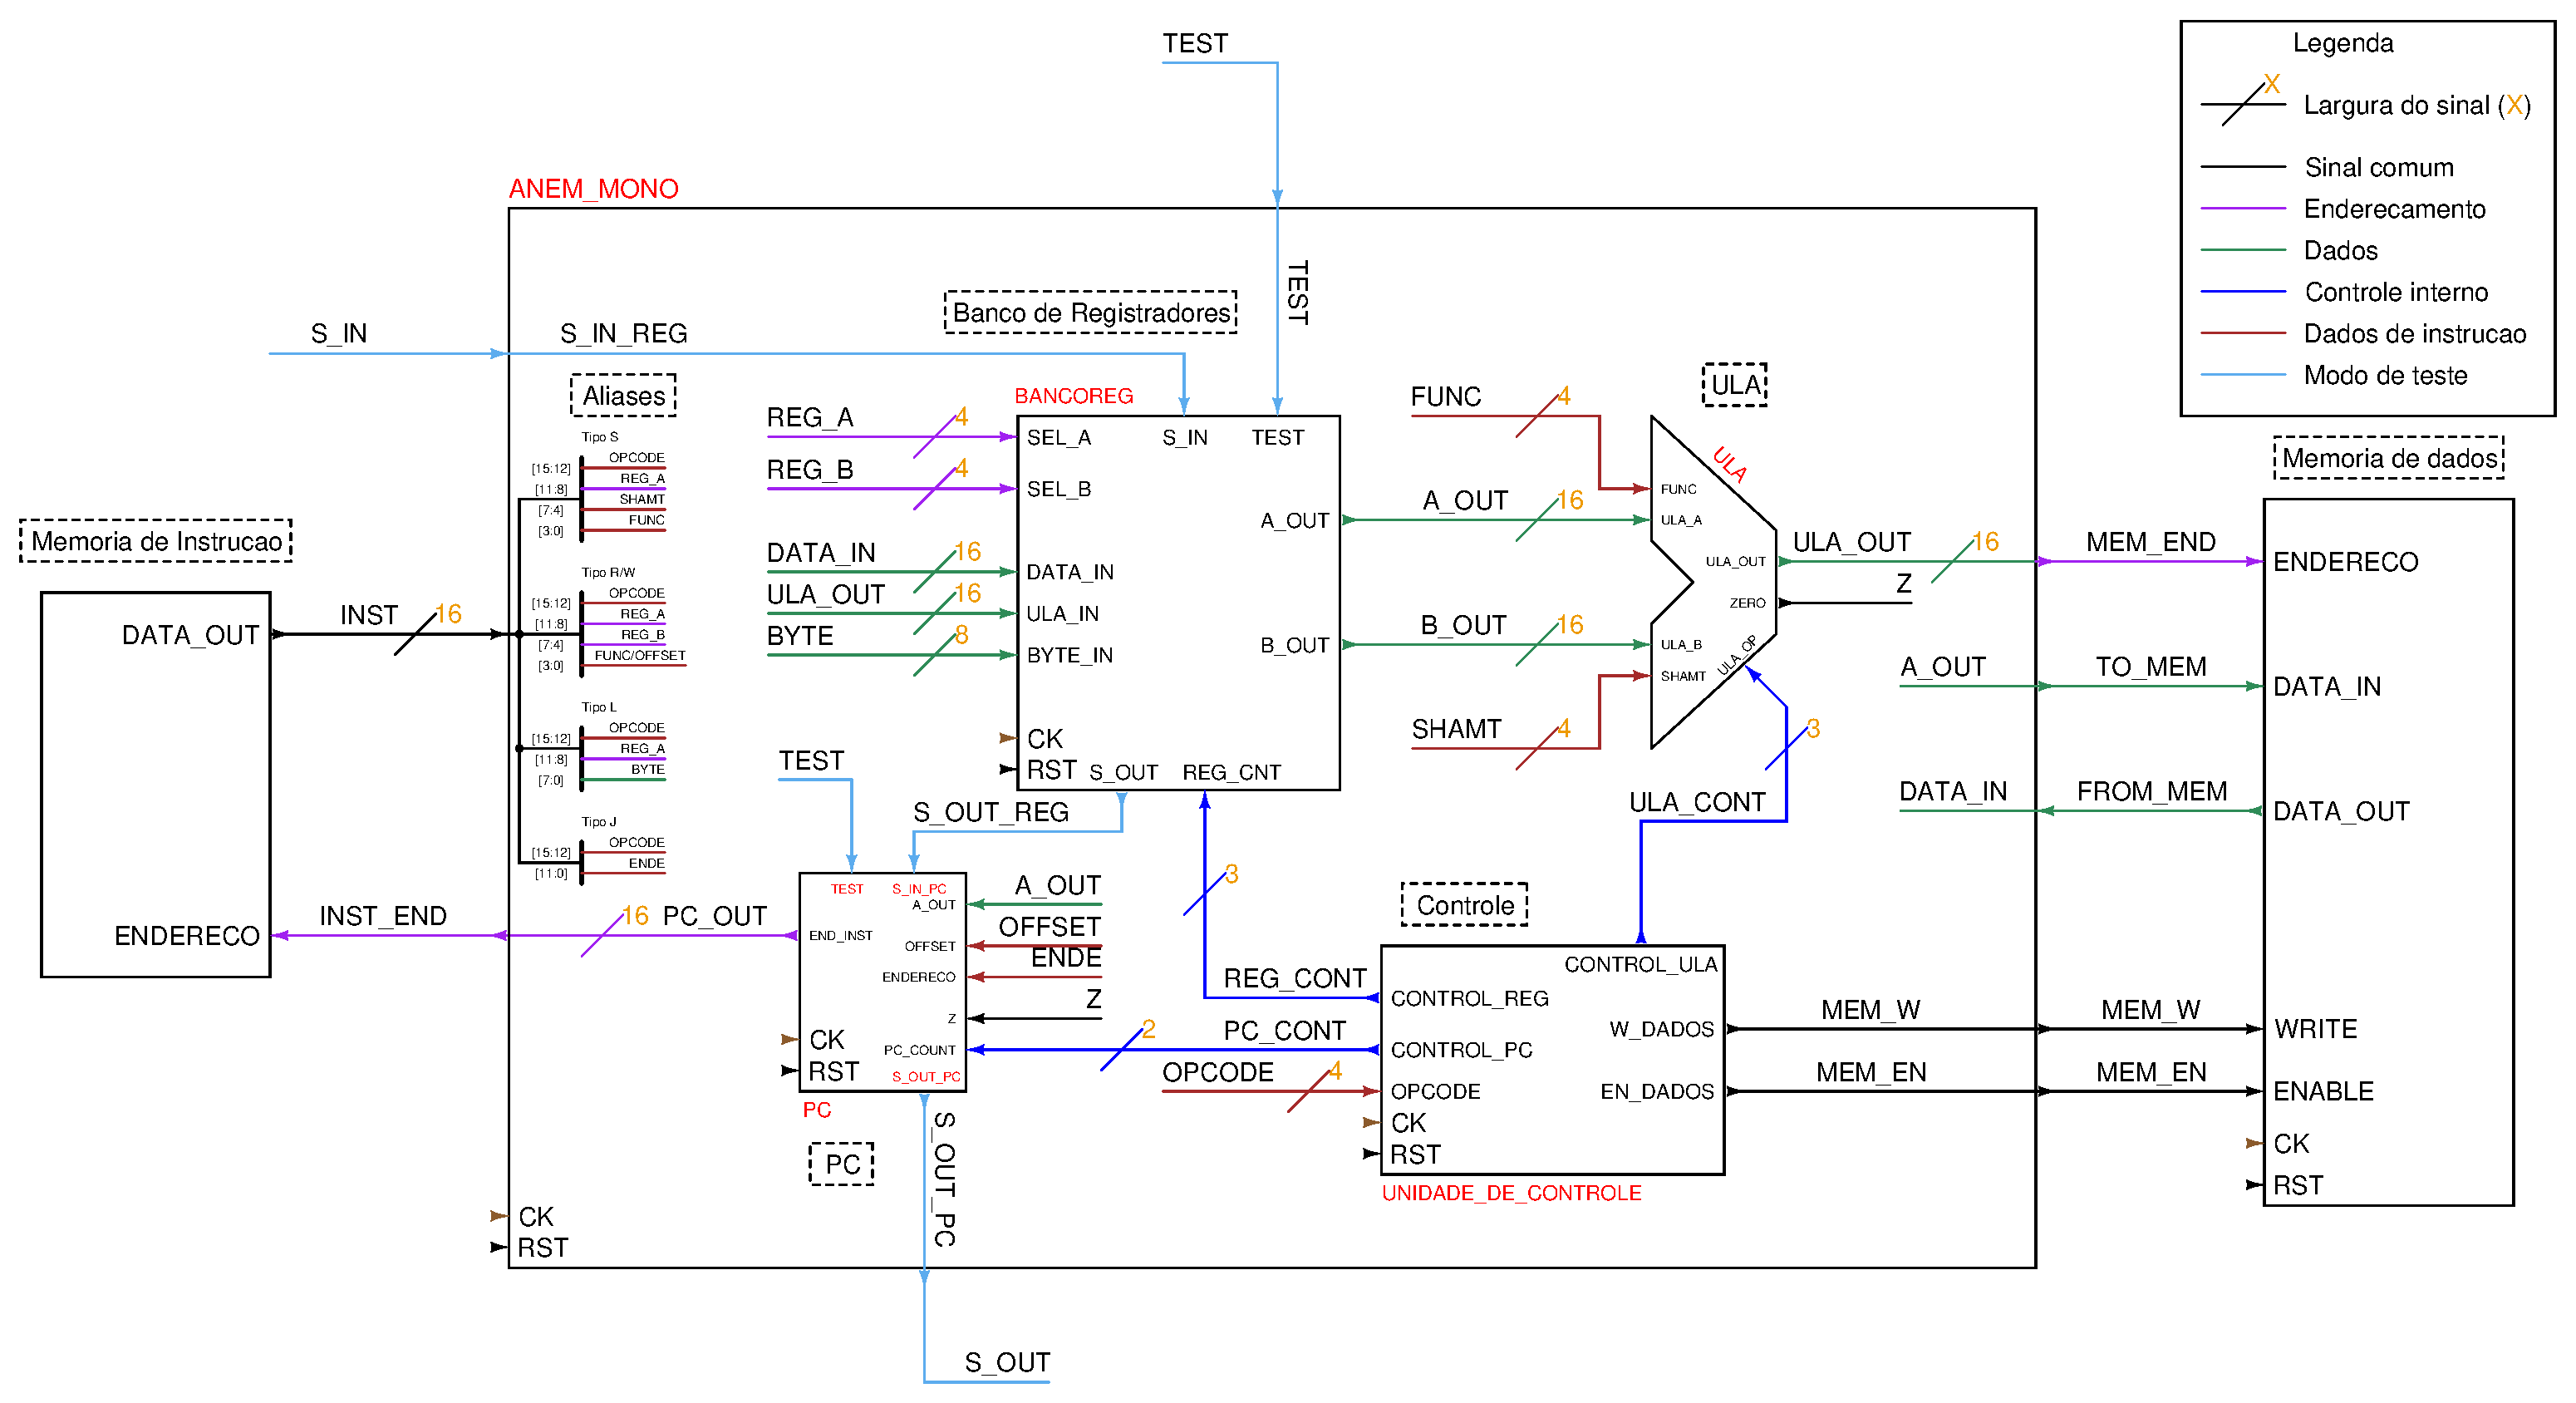
\includegraphics[scale=0.35]{../media/anem_mono_schem.ps}
%\caption{O processador ANEM16 versão mono-ciclo}
%\end{figure}

\subsection{O ANEM-HBUS}

A variação ANEM-HBUS, visa a simplicidade e economia de código, uma vez que os microcontroladores utilizados preferencialmente nos dispositivos HBUS são escolhidos para ter baixo custo e por consequência tem memórias pequenas.

O ANEM-HBUS utiliza palavras de 8-bits. As instruções ainda são de 16-bits. O banco de registradores é composto por 16 registradores de 8 bits e o contador de programa é de 16 bits. O registrador final do banco é fixo no valor zero e é somente para leitura.

Além do banco de registradores, o ANEM-HBUS conta com dois registradores auxiliares, \textbf{HI} e \textbf{LO}.

\subsection{Memória de instrução}

A memória de instrução é um vetor de palavras armazenado em espaço de código, ou seja, é localizado na memória FLASH do microcontrolador. Através de manipulação é possível apagar e re-escrever este conteúdo em tempo de execução. Isto possibilita o \textit{upload} de nova programação com o dispositivo em funcionamento.

O procedimento de \textit{upload} para a execução do microcódigo e re-escreve a memória de instruções. Após isto ser executado com sucesso, o novo microcódigo começa a ser executado. Efetivamente, a \textit{soft-cpu} sofre um RESET.

O upload é conseguido utilizando-se de um \textit{Endpoint} HBUS, conceito já explicado em capítulo anterior. Este endpoint contém a função que realiza a escrita na memória constante de instrução.

\subsection{Instruções disponíveis no microcódigo}

São listadas e discutidas as instruções disponíveis ao usuário. O conjunto de instruções é dividido em tipos, sendo eles:

\begin{itemize}

\item R: Instruções aritméticas
\item S: Instruções de deslocamento
\item J: Instruções de salto incondicional
\item W: Instruções de memória e saltos condicionais
\item L: Instrução para carregamento imediato de valor
\item I: Instrução para geração de interrupções

\end{itemize}

Cada tipo tem um padrão diferente de divisão e utilização dos bits na palavra de instrução. A tabela \ref{tab:inst} detalha as instruções.

\begin{table}[H]
\caption{Instruções disponíveis no microcódigo}
\label{tab:inst}
\begin{tabular}{c c c c}
\hline
Instrução	&	Tipo		&	Descrição\\
\hline
AND			&	R		&	Operação lógica\\
OR			&	R		&	Operação lógica\\
NOT			&	R		&	Operação lógica\\
XOR			&	R		&	Operação lógica\\
ADD			&	R		&	Adição\\
SUB			&	R		&	Subtração\\
MULT			&	R		&	Multiplicação\\
SLT			&	R		&	Compara dois valores\\
DIV			&	R		&	Divisão\\
\hline
SHR			&	S		&	Deslocamento para a direita\\
SHL			&	S		&	Deslocamento para a esquerda\\
ROR			&	S		&	Rotação no sentido da direita\\
ROL			&	S		&	Rotação no sentido da esquerda\\
\hline
J			&	J		&	Salto incondicional\\
JAL			&	J		&	Jump-and-link: salva PC atual nos registradores 13 e 14 e pula\\
\hline
LW			&	W		&	Carrega byte da memória virtual\\
SW			&	W		&	Escreve byte na memória virtual\\
BEQ			&	W		&	Salta em caso de igualdade\\
JR			&	W		&	Salta para endereço contido em registrador\\
\hline
LIW			&	L		&	Carrega valor em registrador imediatamente\\
\hline
INT			&	I		&	Gera interrupção\\
\hline
MFHI			&	M		&	Copia conteúdo do registrador HI\\
MFLO			&	M		&	Copia conteúdo do registrador LO\\
LHL			&	M (M1)	&	Carrega registradores HI e LO\\
LIH			&	M (M1)	&	Carrega registrador HI imediatamente\\
LIL			&	M (M1)	&	Carrega registrador LO imediatamente\\
AIS			&	M (M1)	&	Adiciona valor imediato em HI:LO (com sinal)\\
\end{tabular}
\end{table}

A divisão das palavras de instrução dependendo do tipo de instrução é mostrada a seguir.
%Tabela 1.2 contendo a divisao da palavra de instrucao

\subsubsection{Instruções tipo R}

As instruções tipo R tem estrutura como mostrada a seguir:

\begin{figure}[H]
\centering
\begin{bytefield}[endianness=big,bitwidth=0.035\linewidth]{16}
\bitheader{0-15}\\
\bitbox{4}{OPCODE} & \bitbox{4}{REGA} & \bitbox{4}{REGB} & \bitbox{4}{FUNC}
\end{bytefield}
\caption{Instrução tipo R}
\end{figure}

Estas instruções são operações aritméticas e seus campos são explorados detalhadamente na tabela \ref{tab:ir}. O Opcode das instruções tipo R é 0x0.

\begin{table}[H]
\centering
\caption{Campos da instrução tipo R}
\begin{tabular}{c c p{10cm}}

\hline
Campo	&	Tamanho		&	Função\\
\hline
OPCODE	&	4			&	Informa ao processador o tipo de instrução (R)\\
REGA		&	4			&	Endereço no banco de registradores do operando 1. Também é o destino do resultado\\
REGB		&	4			&	Endereço no banco de registradores do operando 2\\
FUNC		&	4			&	Código que descreve a operação aritmética/lógica a ser realizada\\
\hline
\end{tabular}
\label{tab:ir}
\end{table}

O campo FUNC varia de acordo com a operação a ser realizada. Os valores possíveis e suas correspondentes operações são vistos na tabela \ref{tab:rfunc}.

\begin{table}[h]
\centering
\caption{Instruções tipo R: o campo FUNC}
\begin{tabular}{c l}

\hline
Valor	&	Operação\\
\hline
0x0		&	ADD (adição)\\
0x1		&	SUB (subtração)\\
0x2		&	AND\\
0x3		&	OR\\
0x4		&	XOR\\
0x5		&	NOT\\
0x6		&	MULT (multiplicação)\\
0x7		&	SLT (= 1 se B > A, = 0, c.c.)\\
0x8		&	DIV (divisão)\\
\hline

\end{tabular}
\label{tab:rfunc}
\end{table}

As operações aritméticas tratam os operandos como números sem sinal.

Todas as operações exceto \textbf{DIV} e \textbf{MULT} salvam o resultado da operação no próprio registrador A.

As funções \textbf{DIV} e \textbf{MULT} utilizam os registradores \textbf{HI} e \textbf{LO} da seguinte maneira:

\begin{itemize}

\item \textbf{MULT}: \textbf{HI:LO} = \textbf{REGA} * \textbf{REGB}

\item \textbf{DIV}: \textbf{REGA} = \textbf{HI:LO} \% \textbf{REGB}; \textbf{REGB} = \textbf{HI:LO} / \textbf{REGB};

\end{itemize}

\subsubsection{Instruções tipo S}

As instruções do tipo S são instruções de deslocamento. A estrutura da palavra de instrução é mostrada:

\begin{figure}[H]
\centering
\begin{bytefield}[endianness=big,bitwidth=0.035\linewidth]{16}
\bitheader{0-15}\\
\bitbox{4}{OPCODE} & \bitbox{4}{REG} & \bitbox{4}{SHAMT} & \bitbox{4}{FUNC}
\end{bytefield}
\caption{Instrução tipo S}
\end{figure}

O Opcode destas instruções tem valor 0x1 e seus campos são detalhados a seguir.

\begin{table}[H]
\centering
\caption{Campos da instrução tipo S}
\begin{tabular}{c c p{10cm}}

\hline
Campo	&	Tamanho		&	Função\\
\hline
OPCODE	&	4			&	Informa ao processador o tipo de instrução (S)\\
REG		&	4			&	Endereço no banco de registradores do operando. Também é o destino do resultado\\
SHAMT	&	4			&	Quantidade de deslocamentos realizados\\
FUNC		&	4			&	Código que descreve a operação de deslocamento a ser realizada\\
\hline
\end{tabular}
\label{tab:ir}
\end{table}

\begin{table}[h]
\centering
\caption{Instruções tipo S: o campo FUNC}
\begin{tabular}{c p{6cm}}

\hline
Valor	&	Operação\\
\hline
0x0		&	SHR --- deslocamento a direita\\
0x1		&	SHL --- deslocamento a esquerda\\
0x2		&	ROR --- rotação a direita\\
0x3		&	ROL --- rotação a esquerda\\
\hline

\end{tabular}
\label{tab:sfunc}
\end{table}

As instruções tipo S salvam o resultado das operações no próprio registrador do operando

\subsubsection{Instruções tipo J}

Estas instruções são instruções para a realização de saltos incondicionais. A estrutura da palavra de instrução é mostrada em detalhe:

\begin{figure}[H]
\centering
\begin{bytefield}[endianness=big,bitwidth=0.035\linewidth]{16}
\bitheader{0-15}\\
\bitbox{4}{OPCODE} & \bitbox{12}{ADDRESS}
\end{bytefield}
\caption{Instrução tipo J}
\end{figure}

O campo OPCODE é responsável pela identificação da função da instrução, como já sabido. O campo ADDRESS é o endereço na memória de instrução para qual o processador irá saltar. Em outras palavras esse será o novo valor do \textit{program counter} no próximo ciclo.

As duas instruções utilizadas são descritas:

\begin{table}[H]
\caption{Descrição das instruções tipo J}
\begin{tabular}{c c p{10cm}}
\hline
Instrução 	& 	OPCODE 		&	Descrição\\
\hline
J			&	0x8			&	Salta imediatamente para o endereço dado\\
JAL			&	0x9			&	Jump-and-Link: grava nos registradores 13 e 14 o valor do \textit{program counter} e salta imediatamente para o endereço dado\\
\hline
\end{tabular}
\label{tab:jinst}
\end{table}	 

\subsubsection{Instruções tipo W}

As instruções do tipo W são instruções de salto condicional ou de acesso a memória de programa.

\begin{figure}[H]
\centering
\begin{bytefield}[endianness=big,bitwidth=0.035\linewidth]{16}
\bitheader{0-15}\\
\bitbox{4}{OPCODE} & \bitbox{4}{REGS} & \bitbox{4}{REGD} & \bitbox{4}{OFFSET}
\end{bytefield}
\caption{Instrução tipo W}
\end{figure}

Uma análise dos campos da instrução segue:

\begin{table}[H]
\centering
\caption{Campos da instrução tipo W}
\begin{tabular}{c c p{10cm}}

\hline
Campo	&	Tamanho		&	Função\\
\hline
OPCODE	&	4			&	Informa ao processador o tipo de instrução (S)\\
REGS		&	4			&	Endereço no banco de registradores do registrador fonte\\
REGD		&	4			&	Endereço no banco de registradores do registrador destino\\
OFFSET	&	4			&	Offset para salto ou para ser somado ao endereço de leitura na memória\\
\hline
\end{tabular}
\label{tab:iw}
\end{table}

A terminologia de registrador fonte e registrador destino foi criada para iluminar a operação das instruções.

O registrador \textbf{fonte} é aquele de onde é retirada a informação para a operação de salto ou acesso a memória. No caso das instruções LW e SW, o valor contido no registrador indicado pelo campo da instrução será o endereço da memória a ser lido ou escrito. O registrador destino, no caso da operação de leitura (LW) identifica o registrador no qual será escrito o byte lido da memória. Já para a instrução de escrita (SW), o registrador destino é o registrador que contém o valor a ser escrito na memória virtual. O valor do campo OFFSET é somado ao conteúdo dos registradores que contém os endereços de memória.

Para a operação JR, o registrador de destino perde o sentido e é ignorado, importando apenas o campo de registrador fonte, que deve conter o endereço para onde se deseja saltar. Note que devido a uma limitação das palavras no banco de registrador do ANEM-HBUS, só é possível saltar até a posição 255 da memória de instrução. Esta limitação é relevada, uma vez que o microcódigo não pretende realizar tarefas altamente complexas e por uma questão de limitação em espaço disponível na memória FLASH dos microcontroladores escolhidos, a memória de instrução só é alocada até o tamanho máximo de 256 instruções. O campo OFFSET é somado ao valor do registrador com o endereço da instrução alvo do salto.

Na operação tipo BEQ, os valores contidos nos registradores fonte e destino são comparados, e quando iguais, ocorre o salto para a posição atual do PC mais OFFSET instruções. Mais uma vez, percebe-se uma limitação, já que tendo apenas 4 bits disponíveis, o BEQ é capaz de saltar até apenas 15 instruções a frente da atual. Recomenda-se o uso combinado de uma instrução BEQ que salta para uma instrução tipo J no caso de ser necessário um salto para uma posição mais distante.

\begin{table}[H]
\caption{Descrição das instruções tipo W}
\begin{tabular}{c c p{10cm}}
\hline
Instrução 	& 	OPCODE 		&	Descrição\\
\hline
LW			&	0x5			&	Carrega dados da memória virtual\\
SW			&	0x4			&	Salva dados na memória virtual\\
JR			&	0x7			&	Salta para posição indicada por registrador\\
BEQ			&	0x6			&	Salto condicional dependendo do valor dos registradores\\

\hline
\end{tabular}
\label{tab:winst}
\end{table}	 

\subsubsection{Instrução tipo L}

A instrução do tipo L é a instrução LIW. Os seus campos são mostrados:

\begin{figure}[H]
\centering
\begin{bytefield}[endianness=big,bitwidth=0.035\linewidth]{16}
\bitheader{0-15}\\
\bitbox{4}{OPCODE} & \bitbox{4}{REG} & \bitbox{8}{DATA}
\end{bytefield}
\caption{Instrução tipo L}
\end{figure}

Esta instrução realiza o carregamento imediato de um byte, contido no campo DATA no registrador indicado pelo endereço no campo REG.

\subsubsection{Instrução tipo I}

A instrução do tipo I é a instrução INT. Esta instrução deflagra uma interrupção do barramento HBUS.

\subsubsection{Instruções tipo M}

As instruções do tipo M são destinadas a movimentação e manipulação de dados dos registradores \textbf{HI} e \textbf{LO}. Este tipo de instrução tem alguns subtipos:

\begin{figure}[H]
\centering
\begin{bytefield}[endianness=big,bitwidth=0.035\linewidth]{16}
\bitheader{0-15}\\
\bitbox{4}{OPCODE} & \bitbox{8}{---} & \bitbox{4}{REG}
\end{bytefield}
\caption{Instrução tipo M}
\end{figure}

\begin{figure}[H]
\centering
\begin{bytefield}[endianness=big,bitwidth=0.035\linewidth]{16}
\bitheader{0-15}\\
\bitbox{4}{OPCODE} & \bitbox{4}{MOP} & \bitbox{8}{DATA}
\end{bytefield}
\caption{Instrução subtipo M1}
\end{figure}

\begin{table}[H]
\caption{Descrição das instruções tipo M}
\begin{tabular}{c c p{10cm}}
\hline
Instrução 	& 	OPCODE 		&	Descrição\\
\hline
MFHI			&	0xA			&	Copia conteúdo do registrador HI para REG\\
MFLO			&	0xB			&	Copia conteúdo do registrador LO para REG\\
Subtipo M1	&	0xD			&	Ver tabela abaixo\\

\hline
\end{tabular}
\label{tab:winst}
\end{table}	 

\begin{table}[H]
\caption{Descrição das instruções subtipo M1}
\begin{tabular}{c c p{10cm}}
\hline
Operação 	& 	MOP 		&	Descrição\\
\hline
LHL			&	0x0			&	Carrega registradores HI e LO de DATA[7..4],DATA[3..0]\\
LIH			&	0x1			&	Carrega registrador HI imediatamente com DATA\\
LIL			&	0x2			&	Carrega registrador LO imediatamente com DATA\\
AIS			&	0x3			&	Adiciona valor imediatamente em HI:LO (com sinal)\\

\hline
\end{tabular}
\label{tab:winst}
\end{table}	 

\subsection{A memória virtual}
A memória de dados é mapeada virtualmente a partir dos objetos HBUS declarados pelo dispositivo. Isto dá acesso de leitura e escrita aos objetos. O usuário não tem acesso a memória RAM do microcontrolador, sendo obrigado a limitar-se ao banco de registradores para realizar suas tarefas.

Com o intuito de simplificar a implementação e não impor grandes dificuldades ao processador hóspede (microcontrolador), é assumido que cada objeto HBUS tem um tamanho de 4 bytes.

É uma limitação da especificação HBUS que o objeto tenha no máximo 4 bytes, então não haverá problemas de objetos maiores que os 4 bytes para endereçamento. No caso de o objeto possuir menos de 4 bytes, as tentativas de operações fora deste espaço são simplesmente ignoradas.

Observe que o usuário tem apenas 8 bits para endereçar os objetos, o que dá um total de $\frac{2^8}{4} = 64$ objetos no máximo. Não é esperado que o dispositivo possua essa quantidade de objetos, devido a natureza da especificação HBUS.

\subsection{A operação da máquina virtual}

Um outro termo muito usado para o processador emulado em software é \textit{máquina virtual}.

A máquina virtual que emula o ANEM-HBUS é implementada nos arquivos \textit{microcode.h} e \textit{microcode.c}. 

As funções e estruturas de dados que controlam a operação e o fluxo de dados são descritos brevemente a seguir.

A estrutura de execução é basicamente dividida em duas funções, sendo uma de inicialização e outra que executa um ciclo da máquina virtual.

\subsubsection{Máquina virtual: registradores, estruturas de dados e funções}

Os registradores de dados e também de status do processador são implementados através da estrutura que é mostrada a seguir:

\begin{minted}[linenos]{c}

typedef struct CPUEMU_S
{
	//registradores
	word PC;			//program counter
	
	byte BANK[16];	//banco de registradores
	byte ALUREG; 	//emula a saida da ULA
	
	byte STATUS;		//registrador de status
	
	UCODE_INSTRUCTION INST; //registrador de instrução
	
} UCODE_CPUDATA;

\end{minted}

O processo de inicialização é realizado pela função UCODE\_STARTUP() e os ciclos são gerados pela função UCODE\_CYCLE().

\subsubsection{A função UCODE\_STARTUP()}

Esta função é chamada na inicialização do código do processador hospedeiro. Ela é responsável pela inicialização de todos os registradores da máquina virtual.

Esta função também é chamada no caso de o microcódigo ser atualizado de forma on-line. A máquina virtual é então re-inicializada.

\subsubsection{A função UCODE\_CYCLE()}

Esta função simula os ciclos do processador ANEM-HBUS. Dentro dela são simuladas as etapas de FETCH, DECODE e as operações resultantes,dependendo da instrução que for interpretada no ciclo.

A etapa de FETCH é simulada copiando-se uma palavra de instrução da memória de instrução implementada, em acordo com o valor atual do registrador PC.

A etapa de decode é simulada facilmente e as operações instruídas são realizadas em seguida. Estas operações são realizadas utilizando-se de operadores básicos da linguagem C, no caso de instruções que não envolvam acesso à memória virtual.

No caso de acesso à memória virtual, outras funções, que simulam o acesso de leitura e escrita, são chamadas. Estas funções serão discutidas a seguir.

\subsubsection{A função UCODE\_PAUSE\_()}

Esta função seta um flag no registrador de status que faz com que a operação da máquina virtual cesse. Isto é muito útil no caso de o processador hospedeiro necessitar parar a operação por algum motivo qualquer e é também necessário no caso de ocorrer um update on-line do microcódigo, onde a máquina virtual deve parar para que a memória de instrução possa ser re-escrita.

\subsubsection{A função UCODE\_UNPAUSE()}

Esta função é complementar à anterior, restaurando a operação da máquina virtual.

\subsubsection{As funções UCODE\_LOAD\_DATA() e UCODE\_SAVE\_DATA()}

Estas funções simulam o acesso a memória de programa do ANEM-HBUS, que é a memória virtual onde estão mapeados os dados dos objetos, organizada no esquema já explicado.

Dentro destas funções são chamados os métodos de leitura e escrita especificados pelo próprio objeto, de maneira que a leitura e escrita realizadas pela máquina virtual não diferem de uma leitura/escrita realizada através do barramento HBUS.

\section{O acesso à memória de instrução}

A memória de instrução é por definição alocada em uma parte reservada na FLASH do microcontrolador.
É possível a escrita nesta porção da memória mesmo em tempo de execução.

O acesso neste caso é de escrita e é realizado através de um \textit{endpoint} registrado no dicionário de \textit{endpoints} do dispositivo. Os dados para a memória de instruções são enviados em blocos de 64 bytes conforme a necessidade.

A operação pode ser realizada sem a necessidade de reinicialização do dispositivo, possibilitando a atualização sob demanda do microcódigo, com efeito imediato, através dos procedimentos descritos neste capítulo.


\chapter{Segurança HBUS}

A partir da revisão 1.1 são adicionados mecanismos opcionais para garantir a segurança dos dados trafegados no barramento, incluindo privacidade de objetos e também verificação de identidade do mestre.

\section{Autenticação de mestre}

Este recurso é utilizado para garantir a autenticidade dos comandos enviados aos dispositivos no barramento. Comandos de RESET e escrita em objetos são assinados digitalmente, caso o dispositivo suporte a autenticação.

Isto garante que mesmo no caso de um dispositivo malicioso ser conectado ao barramento, os dispositivos seguros não possam ser instruídos a realizar operações que possam ser danosas ao sistema.

\subsection{O mecanismo de autenticação}

Se o dispositivo suporta autenticação, o mestre deve inserir um bloco de dados após os comandos que necessitam da verificação de identidade.

O dispositivo que suporta autenticação é chamado de \textit{seguro} e o que não suporta de \textit{inseguro}.

Os dispositivos seguros só podem executar os comandos que necessitam de autenticação uma vez que seja verificada a autenticidade da mensagem através do bloco de assinatura.

Um dispositivo seguro descarta os comandos recebidos se eles não possuem o bloco de autenticação ou se a verificação de autenticidade falhou.

Da mesma maneira, os dispositivos inseguros devem ser capazes de receber comandos contendo blocos de autenticação e realizar as tarefas indicadas, ignorando o bloco de autenticação.

\subsection{O método de autenticação}

Para a autenticação são utilizados conceitos similares ao sistema criptográfico de chave pública RSA.

No caso do barramento HBUS, é escolhido um sistema com uma menor complexidade matemática, o sistema criptográfico de Rabin-Williams. Este sistema é muito similar ao sistema RSA, porém pouco conhecido. Ele é equivalente a um sistema RSA com expoente público 2.

As chaves utilizadas são de 1536 bits.

\subsubsection{O sistema criptográfico Rabin-Williams}

O sistema criptográfico de Rabin utiliza o seguinte esquema para suas chaves:

\begin{enumerate}

\item São escolhidos dois números primos p e q, obedecendo: $p \equiv 3 \mod{8}$ e $q \equiv 7 \mod{8}$.

\item $\left({}p,q\right)$ é a chave privada.

\item Calcula-se $n=p\cdot{}q$. $n$ é a chave pública.

\end{enumerate}

\subsubsection{O processo de assinatura}

O mestre realiza este processo todas as vezes que enviar uma mensagem com autenticação.

\begin{enumerate}

\item O mestre calcula $h = H\left({}m|r\right){}$, onde $m$ é a mensagem, $r$ é um número aleatório e $H\left({}\cdot{}\right){}$ é uma função de \textit{hash} pública.

\item Computa-se $U = h^{(q+1)/8} \mod{q}$.
\item Se $U^4 - h \mod{q} = 0$, $e = 1$, c.c. $e = -1$.
\item É calculado $V = \left({}eh\right){}^{(p-3)/8} \mod{p}$.
\item Se $\left({}V^4\left({}eh\right){}^2 - eh\right){} \mod{p} = 0, f = 1$, c.c. $f = 2$
\item É pré-calculado $2^{(3q-5)/8} \mod{q}$. $W = f^{(3q-5)/8}U \mod{q}$.
\item É pré-calculado $2^{(9p-11)/8} \mod{p}.$ $X = f^{(9p-11)/8}V^3eh \mod{p}$.
\item É pré-calculado $q^{p-2} \mod{p}$. Calcula-se $Y = W + q\left({}q^{p-2}\left({}X - W\right){} \mod{p}\right)$.
\item Computa-se $s = Y^2 \mod{pq}$. A assinatura da mensagem é o par $\left({}e,f,r,s\right)$, que é enviado junto a mensagem.

\end{enumerate}

\subsubsection{O processo de verificação}

Esse processo é realizado pelo dispositivo toda vez que recebe uma mensagem com assinatura.

\begin{enumerate}

\item O dispositivo recebe a mensagem juntamente com a assinatura.

\item O dispositivo calcula $efs^2 \mod{pq}$ e $H\left({}m|r\right)$ e verifica se são iguais. Sendo iguais, a assinatura é comprovada

\end{enumerate}

\subsubsection{A função de hash}

A função de hash utilizada é a bem conhecida função SHA-1. A saída da função SHA-1 tem 160 bits de comprimento.

\subsection{O custo da autenticação}

O custo da autenticação é principalmente refletido na quantidade de memória ocupada no dispositivo, tanto de programa quando RAM. Além disto, há o tempo necessário para realizar as verificações, que são baseadas em operações matemáticas um tanto pesadas para dispositivos de 8bits como é o caso dos microcontroladores utilizados no desenvolvimento da pilha HBUS.

Utilizando o processo de autenticação, o overhead de autenticação na mensagem é maior do que a própria mensagem, porém isto é uma questão de segurança e não se pode fazer nada sem comprometer a segurança do sistema.

O bloco de assinatura tem 193 bytes, onde 1 byte é dedicado ao armazenamento das variáveis e,f e r e os 192 bytes restantes são o produto do processo de assinatura realizado pelo mestre (192 bytes = 1536 bits --- tamanho das chaves). 

\section{Autenticação de dispositivo}

O caminho inverso é também possível e desejável em casos que o nível de segurança deve ser maior. No entanto, o sistema de autenticação é assimétrico e a assinatura é muito mais custosa que a verificação. Devido a este fator limitante, a autenticação de dispositivos é possível apenas para dispositivos que utilizem-se de outras soluções mais poderosas que microcontroladores de 8 bits.

Esta é uma funcionalidade futura da especificação HBUS.

\subsection{Requisitos e guia de implementação}

Nesta modalidade de autenticação, cada dispositivo que possuir a capacidade deve ter um par de chaves próprio. Os comandos \hbuscommand{KEYSET} e \hbuscommand{KEYRESET} são utilizados apenas pelo mestre. O dispositivo deve expor sua chave pública através de um objeto invisível contendo o campo PUBKEY.

O mestre, ao realizar a enumeração dos dispositivos, deve verificar as capacidades do mesmo e se ele possuir capacidade de autenticação reversa (autenticação de dispositivo), prosseguir com a obtenção da chave pública.

No entanto, é recomendada a implantação de um esquema de segurança para evitar ataques. O mestre deve ter uma memória permanente de todos os dispositivos e as suas chaves, ou seja, uma vez que um dispositivo se identifica, a chave dele deve ser associada permanentemente ao seu ID único, de forma que se um outro dispositivo tentar emular o ID único e fornecer outra chave pública, o mestre detecte essa irregularidade e tome providências.

\section{Privacidade de objetos}

Este é um mecanismo que permite que os dados relativos aos valores de um objeto, tanto na escrita quando na leitura realizadas pelo mestre sejam criptografados e transmitidos, não permitindo a demais dispositivos que escutam o barramento obter informações sobre o valor do objeto trafegado.

Esta criptografia utiliza a cifra XTEA para simplicidade e as chaves devem ser pré-estabelecidas entre o mestre e o dispositivo. O tamanho de bloco neste processo é de 8 bytes, o que significa que qualquer transmissão de objeto vai ter 8 bytes independente do tamanho do valor contido no objeto.

O mecanismo de codificação e decodificação provê uma verificação automática de validade no caso de recepção de dados e um empacotamento automático no caso de envio de dados.

\subsection{A codificação e decodificação na comunicação}

A máquina de estados de comunicação, ao receber um pacote de escrita ou leitura em um objeto (comandos \hbuscommand{GETCH} ou \hbuscommand{SETCH}), atua normalmente, verificando a validade do comando em questão. Após isto, é verificado se o objeto contém o flag \textit{HBUSOBJ\_CRYPTO}, que informa se o tráfego do valor deste objeto é criptografado ou não. Caso sim ocorre o seguinte procedimento (para escrita):

\begin{enumerate}

\item É verificado se o bloco de dados recebido tem o tamanho correto.
\item Caso o tamanho esteja correto, é realizada a decodificação do bloco.
\item A validade do bloco decodificado é verificada.
\item A função de escrita no objeto é chamada ou os dados são escritos diretamente no ponteiro contido na descrição do objeto, se a verificação teve sucesso

\end{enumerate}

No caso da leitura, o dispositivo é que envia os dados e o procedimento é muito similar ao de escrita e o dispositivo monta o pacote com os dados para verificação na recepção seguindo o padrão.

\subsection{O padrão de verificação de dados}

O padrão de verificação é definido pelo uso de um checksum CRC16.

A estrutura do bloco contendo os dados do objeto e os dados de verificação é vista:

%fazer figura
\begin{figure}[H]
\centering
% XCircuit output "datablock.tex" for LaTeX input from datablock.ps
\def\putbox#1#2#3#4{\makebox[0in][l]{\makebox[#1][l]{}\raisebox{\baselineskip}[0in][0in]{\raisebox{#2}[0in][0in]{\scalebox{#3}{#4}}}}}
\def\rightbox#1{\makebox[0in][r]{#1}}
\def\centbox#1{\makebox[0in]{#1}}
\def\topbox#1{\raisebox{-0.60\baselineskip}[0in][0in]{#1}}
\def\midbox#1{\raisebox{-0.20\baselineskip}[0in][0in]{#1}}
\begin{center}
   \scalebox{1}{
   \normalsize
   \parbox{3in}{
   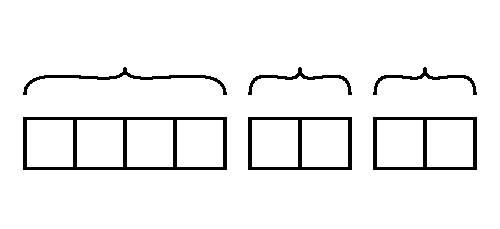
\includegraphics[scale=1]{../media/datablock.ps}\\
   % translate x=512 y=269 scale 0.38
   \putbox{0.39in}{1.12in}{1.20}{DADOS}%
   \putbox{1.72in}{1.12in}{1.20}{SEP}%
   \putbox{2.39in}{1.12in}{1.20}{CRC16}%
   \putbox{0.22in}{0.12in}{1.20}{\centbox{\midbox{0}}}%
   \putbox{0.56in}{0.12in}{1.20}{\centbox{\midbox{1}}}%
   \putbox{0.81in}{0.12in}{1.20}{}%
   \putbox{0.89in}{0.12in}{1.20}{\centbox{\midbox{2}}}%
   \putbox{1.22in}{0.12in}{1.20}{\centbox{\midbox{3}}}%
   \putbox{1.72in}{0.12in}{1.20}{\centbox{\midbox{4}}}%
   \putbox{2.06in}{0.12in}{1.20}{\centbox{\midbox{5}}}%
   \putbox{2.56in}{0.12in}{1.20}{\centbox{\midbox{6}}}%
   \putbox{2.89in}{0.12in}{1.20}{\centbox{\midbox{7}}}%
   \putbox{1.72in}{0.46in}{0.72}{\centbox{\midbox{0xFF}}}%
   \putbox{2.06in}{0.46in}{0.72}{\centbox{\midbox{0xFF}}}%
   } % close 'parbox'
   } % close 'scalebox'
   \vspace{-\baselineskip} % this is not necessary, but looks better
\end{center}

\caption{Bloco de dados para codificação}
\end{figure}

No caso de o objeto não ter o número total de bytes (4), os bytes faltantes devem ser preenchidos com zeros.


\part{Exemplos de implementação e uso}

\chapter{Dispositivos projetados e aplicações}

Neste capítulo são apresentados alguns dispositivos experimentais que foram projetados e sua possível utilização.

\section{Controlador de PWM de 2 canais}

Este é um dos dispositivos sobre o qual foi realizado boa parte do desenvolvimento de todas as especificações HBUS.

O controlador de PWM de 2 canais foi concebido para realizar o controle de intensidade de até 2 fitas de LEDs de comprimento pequeno (até 1m), sendo possíveis as opções de controle por tensão constante ou corrente constante.

Além dos dois canais de saída, o dispositivo possui como entrada um LDR para detecção do nível de luminosidade na região vizinha a placa de circuito impresso e também três chaves de duas posições para uso livre.

O dispositivo é analisado a fundo num capítulo dedicado.

\section{Controlador de PWM com TLC5940}

Este controlador foi desenvolvido juntamente ao controlador de PWM de 2 canais. Sua função é controlar leds ou fitas de leds individuais ou RGB, possibilitando a formação de cores arbitrárias.

O TLC5940 é um circuito integrado fabricado pela Texas Instruments. Ele possui uma interface serial similar à SPI para controle, porém com alguns sinais a mais, sendo necessária a geração de um clock no microcontrolador que implementa a pilha HBUS.

São, no total, 12 saídas de PWM utilizando controle de corrente constante gerenciadas pelo TLC5940.

O software específico a este dispositivo implementa algumas funções interessantes, como controle absoluto ou relativo da luminosidade dos leds e também suporte a mudanças de luminosidades graduais programadas pelo usuário.

\section{Array de sensores}

O dispositivo array de sensores é pertencente a segunda rodada de desenvolvimento. Este dispositivo já incorpora algumas modificações estéticas no desenho da placa de circuito.

O seu objetivo é a captação de variáveis do ambiente em que está localizado para disponibilização ao barramento. Isto pode ser muito interessante e até vital para a automação de um ambiente.

O array de sensores é constituído de sensores de luminosidade ambiente, temperatura e umidade relativa do ar.

\section{Ponte HUB HBUS}

Este é um dispositivo que funciona como ponte entre uma conexão serial comum e o barramento HBUS. É altamente recomendado o uso do mesmo conectado a um computador como o mestre do sistema.

Além da interface de ponte, também é um dispositivo, sendo acessível. Possui algumas entradas e saídas digitais e analógicas.

Na sua segunda versão, o dispositivo é implementado de forma a facilitar a conexão com um computador Raspberry Pi servindo como mestre do barramento HBUS.

As entradas e saídas disponíveis ao mestre do barramento são: 8 entradas/saídas digitais (5 V), 3 entradas analógicas e 4 saídas de PWM. Além disso, através do dispositivo é possível acessar portas de expansão I2C e SPI, para comunicação com dispositivos externos.

A segunda versão do dispositivo contém também um circuito integrado de relógio em tempo real, com bateria para backup, além de monitoramento do consumo do barramento e circuito de proteção e limitação de corrente de saída.


\chapter{Análise detalhada do Controlador de PWM de 2 canais}

Aqui será discutido a fundo o funcionamento deste dispositivo experimental que foi utilizado para o desenvolvimento das especificações HBUS.

\section{Firmware}

O firmware implementa a pilha HBUS com todas as funcionalidades. O código específico do dispositivo controla as funções de geração de PWM no microcontrolador, para acionar o circuito de controle mostrado no esquemático.

\subsection{Os objetos do dispositivo}

O código de declaração dos objetos é mostrado para exemplificar uma implementação.

\begin{minted}[linenos,fontsize=\small]{c}

const HBUSOBJ PWM_CHANNEL_0 = {{HBUSOBJ_WRITE,2,12,"PWM CANAL 00"},0x00,GET_PWM0,SET_PWM0};
const HBUSOBJ PWM_CHANNEL_1 = {{HBUSOBJ_WRITE,2,12,"PWM CANAL 01"},0x00,GET_PWM1,SET_PWM1};
const HBUSOBJ DIP_SWITCH    = {{HBUSOBJ_READ,1,6,"DIP SW"},0x00,GET_SW101,0x00};
const HBUSOBJ LDR_SENS      = {{HBUSOBJ_READ,2,10,"LDR SENSOR"},0x00,GET_LDR,0x00};
const HBUSOBJ FADE_INOUT	= {{HBUSOBJ_WRITE,4,11,"FADE IN/OUT"},0x00,GET_FADEBYTES,SET_FADEBYTES};

\end{minted}

A tabela descreve os objetos em detalhe.

\begin{table}[H]
\centering
\caption{Objetos do controlador de PWM de 2 canais}
\begin{tabular}{c c c c p{6cm}}
\hline
Objeto			&	Endereço		&	Permissão	&	Tamanho	& Descrição\\
\hline
PWM\_CHANNEL\_0	&	0x01			&	W			&	2		& Valor relativo do canal de PWM 1\\
PWM\_CHANNEL\_1 &	0x02			&	W			&	2		& Valor relativo do canal de PWM 2\\
DIP\_SWITCH		&	0x03			&	R			&	1		& Valor das chaves 1,2,3\\
LDR\_SENS		&	0x04			&	R			&	2		& Valor da leitura de luminosidade no LDR\\
FADE\_INOUT		&	0x05			&	W			&	4		& Realiza fade-in / fade-out programável\\
\hline
\end{tabular}
\end{table}

A declaração dos objetos de dispositivo:

\begin{minted}[linenos,fontsize=\small]{c}

const HBUSOBJ * MCU_OBJECTS[HBUS_OBJECT_COUNT] = {&UNIT_INFO, //obrigatorio
						&PWM_CHANNEL_0,
						&PWM_CHANNEL_1,
						&DIP_SWITCH,
						&LDR_SENS,
						&FADE_INOUT
};

\end{minted}

\subsubsection{O objeto zero}

A declaração do objeto zero e sua estrutura HBUSOBJINFO, que identifica o dispositivo é mostrada:

\begin{minted}[linenos,fontsize=\small]{c}

#define S_FAMILY 0x02000000
#define S_NUM    0x00000001

const HBUSOBJLISTINFO OBJECT_INFO = {HBUS_OBJECT_COUNT, HBUS_EP_COUNT, HBUS_INT_COUNT, 
((dword)(S_FAMILY) | (dword)(S_NUM))};
const HBUSOBJ UNIT_INFO = {{HBUSOBJ_READ,sizeof(HBUSOBJLISTINFO),12,"PWM CTRL 2CH"},
&OBJECT_INFO,0x00,0x00};

\end{minted}

\subsection{Os endpoints do dispositivo}

O dispositivo contém apenas um endpoint, que serve para o carregamento do microcódigo HBUS.

\begin{minted}[linenos,fontsize=\small]{c}
const HBUSEP EP_UCODE = {{HBUSEP_WRITE,64,9,"UCODE EP"},UCODE_IMEM,0x00,
UCODE_WRITE_IMEM_BYTE,UCODE_IMEM_WRITE_START,UCODE_IMEM_WRITE_END,0x00,0x00};
\end{minted}

Do código fonte é possível inferir que:

\begin{itemize}

\item O endpoint é de escrita apenas
\item O tamanho de bloco é 64 bytes
\item O nome do endpoint é "UCODE EP"
\item O endpoint tem funções associadas aos eventos de começo e fim de escrita

\end{itemize}

A declaração dos objetos de endpoints:

\begin{minted}[linenos,fontsize=\small]{c}

const HBUSEP * MCU_ENDPOINTS[HBUS_EP_COUNT] = {&EP_UCODE,};

\end{minted}

\subsection{As interrupções do dispositivo}

O controlador de PWM de 2 canais possui apenas a interrupção básica de erro fatal:

\begin{minted}[linenos,fontsize=\small]{c}

const HBUSINT INT_FATAL = {{0x00,5,"FATAL"},0x00};

\end{minted}

A interrupção é gerada em um caso de erro fatal (erro de hardware).

A declaração dos objetos de interrupção:

\begin{minted}[linenos,fontsize=\small]{c}

const HBUSINT * MCU_INTERRUPTS[HBUS_INT_COUNT] = {&INT_FATAL,	};

\end{minted}

\subsection{Exemplo de uso do microcódigo HBUS}

Para melhor ilustrar o uso do microcódigo HBUS, é mostrado um exemplo utilizado no controlador PWM com sucesso.

Este programa é muito simples e funciona na inicialização do dispositivo. Durante a execução normal, o mesmo fica preso num loop infinito e não executa nenhuma ação.

O propósito deste programa é ler as chaves disponíveis na placa do dispositivo e caso as chaves 1 ou 2 estiverem na posição ligado, o canal de PWM 1 ou 2, respectivamente é ativado com valor máximo. Caso as chaves estejam na posição desligado, o dispositivo é inicializado com o respectivo canal PWM no valor mínimo.

O código fonte mostrado apenas cobre a chave e canal número 1.

O programa em ANEM-assembly contém apenas 10 instruções e é mostrado a seguir:

\begin{minted}[linenos]{nasm}

LIW	0,	0x0C
LW	$0,	1
LIW	2,	0x01
NOT	$1
AND	$1,	$2
BEQ	$1,	$2,		2
J	0x00A
LIW	0,	0x05
LIW	1,	0xFF
SW	$1,	$0
J	0x00A

\end{minted}

Este código mostrado resulta nas instruções mostradas abaixo:

\begin{table}[H]
\centering
\caption{Instruções no programa exemplo (microcódigo)}
\begin{tabular}{c c p{10cm}}
\hline
Posição	&	Palavra		&	Descrição\\
\hline
0		&	0xC00C		&	Carrega o endereço do objeto correspondente as chaves de seleção no reg. 0\\
1		&	0x5100		&	Copia o valor do objeto no endereço (valor do reg. 0) para o reg. 1\\
2		&	0xC201		&	Carrega a máscara da chave de interesse (0x01) no reg. 2\\
3		&	0x0105		&	Inverte o conteúdo do registrador 1\\
4		&	0x0122		&	Realiza AND com os conteúdos dos registradores 1 e 2 e coloca o resultado no reg 1\\
5		&	0x6122		&	Pula para a posição 5+2=7 se o conteúdo do reg. 1 = reg 2\\ 
6		&	0x800A		&	Pula para a posição 0x00A (se a condição anterior falhou)\\
7		&	0xC005		&	Carrega endereço do objeto de PWM 1 no reg. 0\\
8		&	0xC1FF		&	Carrega valor para escrever no byte (0xFF) no reg. 1\\
9		&	0x4010		&	Grava valor no byte do objeto\\
A		&	0x800A		&	Pula para 0x00A (loop infinito)\\
\hline
\end{tabular}
\end{table}

\subsection{O conteúdo do arquivo de código específico}

Este arquivo contém o código específico ao dispositivo que implementa as funções de escrita e leitura dos objetos do dispositivo referenciadas na declaração dos mesmos. Ele é simples e é mostrado na íntegra a seguir:

\begin{minted}[linenos,fontsize=\small]{c}

#include "ledctl/ledctl.h"
#include "serial/serial.h"
#include <string.h>

dword TIMECOUNTER = 0;
dword LED_LASTCYCLE = 0;
dword LAST_DEBOUNCE = 0;

static word PWM0_VALUE = 0x0000;
static word PWM1_VALUE = 0x0000;

static byte SWSTATE = 0x00;

word LDR_LAST = 0x0000;

typedef struct {
	byte FADESTATUS;
	union{
		word w;
		byte b[2];
	} FADETO;
	byte FADEINCR;
} FADES;

FADES FADE;

#pragma MESSAGE DISABLE C5703

static void PWM_REFRESH(void)
{
	TPMC1V = PWM0_VALUE;
	TPMC0V = PWM1_VALUE;
}

void LEDCTL_STARTUP(void)
{
	//PWM SETUP
	
	  TPMSC = 0x00;
	  TPMC1SC = 0x3C;
	  TPMC0SC = 0x3C;
	  PWM0_VALUE = 0xFFFF;
	  PWM1_VALUE = 0xFFFF;
	  TPMMOD = 0x1F3F;
	  
	  PWM_REFRESH();
	  
	  TPMSC = 0x08;
	  
	  FADE.FADESTATUS = 0;
	  FADE.FADETO.w = 0;
	  FADE.FADEINCR = LEDCTL_FADE_INCR;
	  
	  SWSTATE = SW101;
}

void LEDCTL_CYCLE(void)
{
	
	static byte LAST_SWSTATE = 0x00;
	
	if ((LED_LASTCYCLE + LEDCTL_CYCLE_T) > TIMECOUNTER) return;
	
	if (!(FADE.FADESTATUS & FADESTATUS_FADERUN)) return;
	
	if (FADE.FADESTATUS & FADESTATUS_FADEIN)
	{
		
		if (FADE.FADESTATUS & FADESTATUS_FADE0)
			if (FADE.FADETO.w <= PWM0_VALUE) {
				if (PWM0_VALUE >= (FADE.FADETO.w + FADE.FADEINCR)) PWM0_VALUE -= FADE.FADEINCR;
				else PWM0_VALUE = FADE.FADETO.w;
			}
		
		if (FADE.FADESTATUS & FADESTATUS_FADE1)
			if (FADE.FADETO.w <= PWM1_VALUE) {
				if (PWM1_VALUE >= (FADE.FADETO.w + FADE.FADEINCR)) PWM1_VALUE -= FADE.FADEINCR;
				else PWM1_VALUE = FADE.FADETO.w;
			}
		
	}else if (FADE.FADESTATUS & FADESTATUS_FADEOUT)
	{
		
		if (FADE.FADESTATUS & FADESTATUS_FADE0)
			if (FADE.FADETO.w <= PWM0_VALUE) {
				if (PWM0_VALUE <= (FADE.FADETO.w - FADE.FADEINCR)) PWM0_VALUE += FADE.FADEINCR;
				else PWM0_VALUE = FADE.FADETO.w;
			}
		
		if (FADE.FADESTATUS & FADESTATUS_FADE1)
			if (FADE.FADETO.w <= PWM1_VALUE) {
				if (PWM1_VALUE <= (FADE.FADETO.w - FADE.FADEINCR)) PWM1_VALUE += FADE.FADEINCR;
				else PWM1_VALUE = FADE.FADETO.w;
			}
		
	}
	
	PWM_REFRESH();
	
	if ((PWM1_VALUE == FADE.FADETO.w) || (PWM0_VALUE == FADE.FADETO.w)) 
		FADE.FADESTATUS &= ~FADESTATUS_FADERUN;
	
	//DEBOUNCE
	if (SW101 != SWSTATE)
	{
		
		if ((LAST_DEBOUNCE + LEDCTL_DEBOUNCE_T) > TIMECOUNTER)
		{
			
			SWSTATE = SW101;
			
			LAST_DEBOUNCE = TIMECOUNTER;
			
		}
		
	}
}

void SET_PWM0(void * data, int size)
{
	
	PWM0_VALUE = ~(*(word*)(data));
	
	PWM_REFRESH();
	
}

void SET_PWM1(void * data, int size)
{
	
	PWM1_VALUE = ~(*(word*)(data));
	
	PWM_REFRESH();
	
}

void SET_FADEBYTES(void * data, int size)
{
	
	FADE.FADESTATUS = (*(byte*)data);
	FADE.FADETO.b[0] = ~(*((byte*)data+1));
	FADE.FADETO.b[1] = ~(*((byte*)data+2));
	FADE.FADEINCR = (*((byte*)data+3));
	
	if (!FADE.FADEINCR) FADE.FADEINCR = LEDCTL_FADE_INCR;
	
}

void * GET_FADEBYTES(void)
{
	static FADES fret;
	
	(void)memcpy(&fret,&FADE,4);
	
	fret.FADETO.w = ~fret.FADETO.w;
	
	return (void*)&fret;
}

void * GET_SW101(void)
{

	return (void*)(&SWSTATE);
	
}

void * GET_PWM0(void)
{
	
	return &PWM0_VALUE;
	
}

void * GET_PWM1(void)
{
	
	return &PWM1_VALUE;
	
}

\end{minted}

\section{Hardware}

O hardware deste dispositivo é composto apenas do básico para a implementação da pilha HBUS e as funções de hardware requeridas nesse caso (controle PWM).

O bloco de controle PWM é configurado no momento da montagem da placa e pode ser utilizado como um controle de tensão constante ou corrente constante, dependendo da configuração.


\begin{figure}[H]
\centering
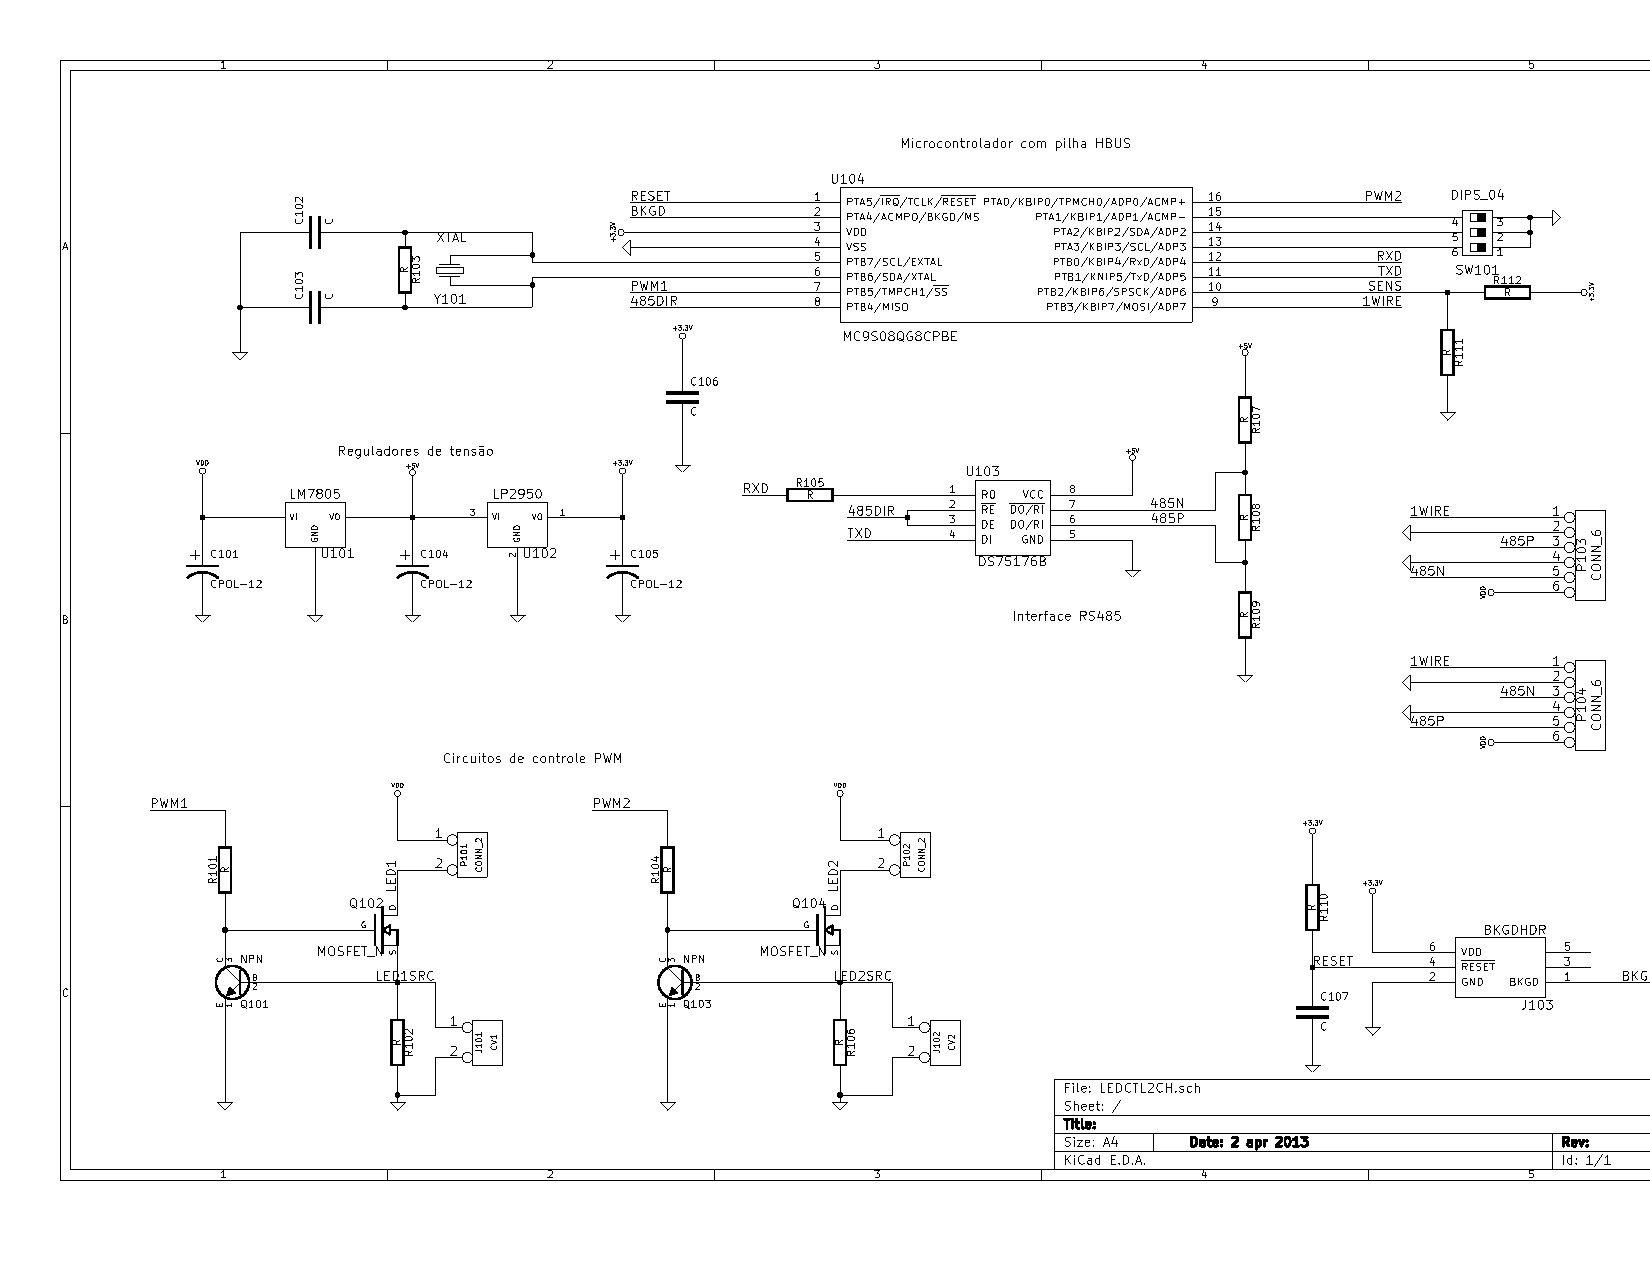
\includegraphics[scale=0.75]{../media/LEDCTL2CH.pdf}
\caption{Esquemático Controlador PWM 2 canais}
\end{figure}


\appendix
\chapter{Unidades padrão no HBUS}

A especificação HBUS, através do uso de objetos invisíveis e utilizando a sintaxe da seção \ref{sec:hiddenobj}, através do campo UNIT, implementa algumas unidades padrão do SI, para melhor visualização dos dados disponibilizados pelos dispositivos.

\section{Unidades de medidas}

As unidades suportadas pelo sistema são um conjunto de reduzido de unidades comuns utilizadas no SI.

\begin{table}[H]
\centering
\caption{unidades padrão no HBUS}
\begin{tabular}{l l l}
\hline
Unidade		&	Símbolo SI	&	String HBUS\\
\hline
\textit{volt} & V			&	V\\
\textit{ampère} & A			&   A\\
\textit{watt}   & W			&   W\\
\textit{pascal} & Pa			&   Pa\\
\textit{graus Celsius} & $^{\circ} C$ & C\\
\textit{ohm}		& $\Omega$	&	R\\
\end{tabular}
\end{table}

\section{Prefixos suportados}

Vários prefixos são suportados para uso conjunto com as unidades. Estes prefixos devem vir antes da unidade, sem espaços.

A tabela abaixo lista os prefixos suportados e o caractere para uso nos dispositivos.

\begin{table}[H]
\centering
\caption{prefixos suportados no HBUS}
\begin{tabular}{l c c l}
\hline
Prefixo		&	Símbolo SI	&	Caractere HBUS	&	Potência\\
\hline
%pico			&	p			&	p				&	$10^{-12}$\\
%nano			&	n			&	n				&	$10^{-9}$\\
micro		&	$\mu$		&	u				&	$10^{-6}$\\
mili			&	m			&	m				&	$10^{-3}$\\
kilo			&	k			&	k				&	$10^3$\\
mega			&	M			&	M				&	$10^6$\\
\hline
\end{tabular}
\end{table}


\end{document}